\documentclass[11pt,a4paper]{article}

\usepackage[T1]{fontenc}
\usepackage[utf8]{inputenc}
\usepackage{lmodern}
\usepackage[margin=2.4cm]{geometry}
\usepackage{amsmath,amssymb,amsthm,bm,mathtools}
\usepackage{booktabs,array,tabularx,multirow}
\usepackage{graphicx}
\usepackage{enumitem}
\usepackage{xcolor}
\usepackage{tikz}
\usetikzlibrary{arrows.meta,decorations.pathreplacing,calc,patterns,positioning}
\usepackage{xr-hyper}
\usepackage[colorlinks=true,linkcolor=teal!70!black,citecolor=teal!70!black,urlcolor=teal!70!black]{hyperref}
\usepackage{caption}
\captionsetup{font=small,labelfont=bf}
% Labels of the main text are referenced with the prefix M-.
\externaldocument[M-]{paper1_short}[paper1_short.pdf]

\theoremstyle{plain}
\newtheorem{theorem}{Theorem}
\newtheorem{proposition}{Proposition}
\newtheorem{lemma}{Lemma}
\newtheorem{corollary}{Corollary}
\theoremstyle{definition}
\newtheorem{definition}{Definition}
\newtheorem{counterexample}{Counterexample}
\theoremstyle{remark}
\newtheorem{remark}{Remark}

\usepackage{etoolbox}
\makeatletter
\patchcmd{\l@section}{1.5em}{2.4em}{}{}
\makeatother
\renewcommand{\thesection}{S\arabic{section}}
\renewcommand{\thetable}{S\arabic{table}}
\renewcommand{\thefigure}{S\arabic{figure}}
\renewcommand{\theequation}{S\arabic{equation}}
\renewcommand{\thetheorem}{S\arabic{theorem}}
\renewcommand{\theproposition}{S\arabic{proposition}}
\renewcommand{\thelemma}{S\arabic{lemma}}
\renewcommand{\thecounterexample}{S\arabic{counterexample}}
\renewcommand{\theremark}{S\arabic{remark}}

\setlength{\parskip}{0.4em}
\setlength{\parindent}{0pt}
\newcommand{\nj}{\textsc{nj}}
\newcommand{\nh}{\textsc{nh}}
\newcommand{\tcross}{\tau_{\mathrm{cross}}}
\newcommand{\pred}{\operatorname{pred}}
\newcommand{\R}{\mathbb{R}}
\newcommand{\Pb}{\mathcal{P}}
\newcommand{\Psim}{\Pb^{\mathrm{sim}}}
\newcommand{\Pd}{\Pb_\Delta}
\newcommand{\Fpi}{\overline F_\Pi}
\newcommand{\I}{\mathcal I}

\title{\textbf{Supplementary material for}\\[0.3em]
\textbf{Scheduling a Shared Mobile Head Across Parallel Conveyors with Endogenous Blocking}}
\author{laser-conveyor-optimization\\\small\url{https://github.com/juanlopez-gif/laser-conveyor-optimization}}
\date{November 2026 --- supplement to the short version of draft 1.3 (version 0.7.42)}

\begin{document}
\maketitle

This file contains the material moved out of the main text: the finer comparisons with
the literature, the complements of the formulation and of the online model, the
time-indexed MILP, all proofs, the design study of the search, the details of the learned
policy, all development results, and further material of the confirmatory evaluation.
Sections, tables, figures, equations and statements numbered with a prefix S belong to
this file; numbers without the prefix refer to the main text. Most of the text is taken
verbatim or near-verbatim from draft~1.3.

\setcounter{tocdepth}{1}
\tableofcontents
\clearpage

%====================================================================
\section{Extended related work}\label{sec:relatedfull}
%====================================================================
This section reproduces the full comparison with the literature that Section~\ref{M-sec:related} condenses.

\textbf{Picking and sorting from moving conveyors.} With one arm over one belt and
Poisson arrivals, \cite{S02_Han2020} sequence the reachable objects by dynamic
programming and show that greedy rules (first-in, nearest-first) are not optimal in
general; the belt never stops and objects that leave the window are lost. Sorting on a
moving belt \cite{S01_Mattone2000} and value-aware sorting with availability windows
\cite{S05_Kokkalis2026} share that setting. With several arms, \cite{S03_Nielsen2023}
batch items from an infeed belt into tray lanes inside a 1.8~s decision budget, and
\cite{S04_Schettini2023} schedule identical robots along input and output conveyors by
row generation and local search with cameras that see items 5--10~s ahead. A robot arm
that always takes the foremost item of one of several accumulating infeeds, with no
release times and no belt stops, reduces makespan to empty travel and is polynomial for a
fixed number of infeeds \cite{Li2026}. In all of these the windows of the items to be
picked are exogenous; where conveyor motion is itself a decision, as for the output
conveyor of \cite{S04_Schettini2023}, it is a separate control lever rather than a
consequence of the processing. In our cell the windows are set by the schedule itself.

\textbf{Interception of moving targets.} The moving-target travelling salesman problem
\cite{S06_Helvig2003}, its formulations with visibility windows \cite{S07_Stieber2022}
and the mixed-integer conic formulation over a graph of convex sets \cite{S08_Philip2024}
give exact models of a single agent intercepting targets with exogenous, constant
velocities, offline. Our formulation uses the same interception geometry with endogenous
motion: a belt's odometer stops while its part is processed or blocked.

\textbf{Blocking in conveyor systems.} Blocking as a schedule-dependent loss appears in
packaging machines whose devices obstruct each other \cite{S10_Briskorn2025} and in a
warehouse where full crane buffers stop the upstream conveyors \cite{S11_SalviaHornos2026},
both minimised offline. Our objective charges the blocking events and their duration
inside the online dispatching problem. Single-machine scheduling with release dates, from
which our complexity result is inherited, is classical \cite{Lenstra1977,Schrage1968,Baker1974}.

\textbf{Mixed-model assembly lines.} Work that cannot be finished inside a station is
either left to utility workers while the line keeps moving \cite{Yano1991,Tsai1995,Sarker2001},
or stops the conveyor until it is done \cite{Xiaobo2000,Tamura2011}. In the first case the
windows are exogenous and, for a given launch sequence, a first-come-first-served
allocation minimizes the work overload \cite{Yano1991}; the risk of a stop is measured by
how far downstream the operator drifts, not by a stop of the line \cite{Tsai1995}; and line
parameters such as the launch interval and the station lengths can be optimized jointly
with the sequence \cite{Sarker2001}. In the second case a stop halts every station at once
and shifts every later product, the makespan exceeds the line-stoppage time by a constant
\cite{Tamura2011}, and sequencing is already strongly NP-hard for one station
\cite{Tsai1995,Xiaobo2000}. In all of them each station has its own worker and the decision
is the launch order, fixed offline. Our cell differs in the interaction: one mobile head
serves several parallel belts, every service stops only the belt it serves, so that the
relative positions of the belts change with each decision, and the decision is taken online
among the parts in view (Section~\ref{M-sec:example} gives a two-belt example). The
variant with all conveyors stopped by every service ($\sigma\equiv1$) recovers a line-wide
stop.

\textbf{Rollout and learned dispatching.} The look-ahead of Section~\ref{M-sec:search} is a
rollout \cite{M02_Bertsekas1997}: a base policy simulated from each candidate, with the
base choice kept on ties. In conveyor cells, a rollout has been used to choose the
acceleration of the output conveyor of a robotic picking line, with simulated futures
truncated at 20--80~s \cite{Righettini2025}, and sampled completions of the unseen part of
the infeed queues, solved and combined by a vote on the first action, bring an item-sorting
robot close to its full-information optimum \cite{Li2026}. Learned dispatching policies trained from search or from expert
schedules include policy-gradient dispatching with objective-aligned rewards
\cite{S19_Zhang2020,S21_Sun2023}, offline learning from constraint-programming schedules
\cite{S20_VanRemmerden2025}, look-ahead-based learning for robotic flow shops
\cite{S14_Kim2023}, action masking \cite{M04_Huang2022,S18_Wei2024}, and learned control
of conveyor-fed robotic cells \cite{S15_Zisgen2025,S16_Drijver2023,S17_Drakaki2017,S12_Wang2004,S13_Li2020}.
The training loop used here, a search that improves on the current policy and a policy
fitted to the search's choices, repeated, is expert iteration \cite{Anthony2017,Silver2018},
with the state-distribution correction of \cite{Ross2011}; what is specific to this paper
is the expert (a scenario rollout scored on every part) and the observation, on one
training chain per network size, that changing the expert moved the policy's score while
larger networks did not score detectably better; size, episodes and iterations are confounded in
those runs. Learning directly from the reward with a
policy-gradient method \cite{Schulman2017} on the same representation is the baseline
that the question ``what does learning from the search add'' calls for; the project's
earlier attempt used another representation and action space (Section~\ref{sec:rlhistory}),
and a baseline on the present one is reported in Section~\ref{sec:ppo}.

%====================================================================
\section{Complements of the formulation and of the online model}\label{sec:formdetails}
%====================================================================
\subsection{Travel path and objectives}
With simultaneous axes the head moves diagonally until one axis
arrives and then straight, and its path length is
$\ell(P,Q)=\max(\Delta y+c_x\Delta x,\ \Delta x+c_y\Delta y)$ with
$c_x=(\sqrt{v_x^2+v_y^2}-v_y)/v_x$ and $c_y$ symmetric, convex in $\Delta x$ for fixed
$\Delta y$ (used in Section~\ref{app:milp}). Both travel-time models of \eqref{M-eq:tau} are
metrics (weighted $\ell_\infty$ and $\ell_1$ norms). In (C2), the head, leaving
$P_{\pi(i)}$ at $C_{\pi(i)}$, reaches the point where the moving part will be at
$S_{\pi(i+1)}$ no later than the part (it may wait there); by the triangle inequality,
\eqref{M-eq:C2} implies $S_j\ge C_i+\tau(P_i,P_j)$ for every pair with $i$ before $j$. In (C4),
since $D_k$ is non-decreasing the condition $D_{k(j)}(t)-E_j\le b$ for all $t\le S_j$ is
equivalent to $X_j\le b$, already in (C1). Dropping (C5) gives the relaxed model $\Pb^R$ in
which belts may also be stopped voluntarily.

All objectives are minimized: the makespan $C_{\max}=\max_jC_j$, the total flow time
$\sum_j(C_j-r_j)$, the total waiting time $\sum_j(S_j-r_j)$, the maximum lateness
$L_{\max}=\max_j(C_j-d_j)$ for due dates $d_j$, the head's travel distance, the conveyor
downtime $\sum_k\bigl(T-D_k(T)/v_k\bigr)$ with $T$ the exit time of the last part, and the
throughput $n/C_{\max}$ (the one quantity to be maximized; for a fixed number of parts
maximizing it is equivalent to minimizing the makespan). The penalty weights carry units: $\lambda_N$ is seconds per event
and $\lambda_T$ is dimensionless, since $T_B$ and the flow time are both in seconds. A part that reaches the end of the laser zone unprocessed stops
its whole conveyor by (C4)--(C5); the delays it causes are inside the $C_j$, but a blocked
conveyor has further costs in the cell (restart, accumulation upstream, risk for the
upstream process), so it is penalized explicitly. $B_j$ is well defined, since by (C4) the
belt stops exactly when $x_j=b$, and the blocked duration of part $j$ is $(S_j-B_j)^+$.
Since $\Pi\ge0$, every lower bound of the mean flow time is a lower bound of $\Fpi$. The
flow-time and blocking components of every result are reported separately.

\subsection{Pre-positioning, action modes and the decoder}
Constraint (C2) allows the head to move towards a part \emph{before} it reaches the laser
zone: it may pre-position at $(a,y_k)$ and wait. Since (C7) only removes schedules, $\Pb$ is a relaxation
of $\Psim$: its optimum is a lower bound on the cost of every schedule a non-anticipating
controller can produce, and the gap between the two optima measures what the restriction
(C7) costs under full knowledge of the instance (a single part arriving at $t=0$
completes at $5.83$~s in $\Pb$ and at $7.19$~s in $\Psim$); it is not the value that an online
controller obtains from pre-positioning, which Section~\ref{M-sec:confirm} and the companion
paper measure as paired contrasts between policies. The cell's two action modes
are, with $\mathcal R(t)$ the ready unassigned parts (inside the zone) and $\mathcal U(t)$
the unassigned parts in the entry zone of a running belt: \texttt{none}, candidates
$\mathcal R(t)$, whose schedules satisfy the constraints of $\Psim$ (a non-idling policy in
this mode does not reach every schedule of $\Psim$: a deliberate wait for a part that is
not yet ready while another part is ready is feasible for $\Psim$); and \texttt{when\_idle}, candidates $\mathcal R(t)$
if non-empty and $\mathcal U(t)$ otherwise, feasible for $\Pb$. A \emph{dispatch event} is an
instant at which the head is free and the candidate set is non-empty; with a single
candidate the dispatch is forced, and a \emph{decision epoch} (Section~\ref{M-sec:online})
is a dispatch event with at least two candidates. Commitments are
irrevocable until processing starts, except that under \texttt{when\_idle} a commitment to
an entry-zone part $j$ is revoked at the first instant $t'$ with $\mathcal R(t')\ne\emptyset$,
$j\notin\mathcal R(t')$; the head keeps its position, nothing else is charged, and a new
epoch occurs at $t'$ with candidates $\mathcal R(t')$. Physically, \texttt{when\_idle}
requires the camera to see the entry zone.

The offline problem with full knowledge of the arrivals is the clairvoyant benchmark; the
cell's problem is its online version. A time-indexed MILP of $\Pb$ is given
in Section~\ref{app:milp}: exact up to the step for the flow-time and makespan
objectives, and, for the blocking penalty, an approximation whose witness is specified
there but not validated against the continuous model; it is tractable on small instances
and inside a rolling horizon. Once the order $\pi$ is fixed,
the earliest schedule compatible with (C1)--(C5) and (C7) is obtained by a deterministic
forward pass $\Phi:\pi\mapsto(S,u)$, which is what the cell's simulator computes for a
fixed sequence; $\min_\pi\Fpi(\Phi(\pi))$ is a permutation problem, but $\Phi$ is a
heuristic restriction of $\Psim$ (Proposition~\ref{prop:delay} shows that a delay cannot
pay through the head's travel alone; whether it can pay through the belt's motion, which
brings a part closer to the head, is left open, Section~\ref{app:special}), and dynamic programming over (processed set, last part) is not
exact, because the odometers depend on the whole history.

\subsection{Return, state and the cost identity}
The undiscounted return of an
episode, taken as the whole-episode accounting identity (the return a learner stores
from its first discretionary action is minus the final cost plus the cost already accrued
at that decision, below), is $-n\,\Fpi$, i.e.\ minus the total cost of the episode: a learner that
maximizes the undiscounted return minimizes the total cost, a discounted proxy would
not, and because $n$ varies between episodes the return weights an episode by its
number of parts, which is not the per-part cost $\Fpi$ of \eqref{M-eq:J}; the two
objectives are stated where each is used (Sections~\ref{M-sec:general} and
\ref{sec:ppo}).

\textbf{State, observation and the cost identity.} The state of the process is the full
state of the cell: the head, the belts' odometers and stops, every part released,
including those waiting in the hidden queue upstream of the feed point, and, under
bursty arrivals, the phase of the source; between epochs it evolves under the action and
the arrival process. A policy acts on the observation $\I_t$ of Section~\ref{M-sec:info},
which omits the hidden queue and the source's phase, so $\I_t$ need not be a Markov
state of the process; every policy of this paper is a function of $\I_t$, with the
audited exception of the legacy comparators of Section~\ref{M-sec:confirm}, whose
tie-break used $r_j$ (below; they were rerun afterwards with the observable key), and nothing below assumes more. The identity between return and cost covers the whole episode:
$n\Fpi=c(0,t_1)+\sum_{i=1}^{m-1}c(t_i,t_{i+1})+c(t_m,T)$, with $t_1$ the first decision
epoch, $t_m$ the last and $T$ the instant the last part leaves; the first term is the
cost of the forced initial segment (waiting for the first part, single-candidate
dispatches), which no decision influences, and the last term, the draining after the
last decision, still depends on the last action although no decision follows it; both
are part of the episode's cost. An episode with at least one arrival and no decision
epoch (a single part, or forced dispatches only) has a total cost $c(0,T)>0$ and no $t_1$
or $t_m$ to introduce; with no arrival the total cost is zero and the per-part objective
$\Fpi$ is undefined. The learners of Sections~\ref{M-sec:policy} and \ref{sec:ppo} attribute
to each decision the cost accrued until the next one and the terminal segment to the
last decision, and score the forced initial segment in the episode cost. An episode
with no arrival has zero total cost and an undefined per-part cost $\Fpi$: it is
excluded from every per-part mean and reported separately where it occurs
(Section~\ref{sec:ppo}).

\subsection{Tie-break audit on development realizations}
Rules that rank candidates by travel time compare the times rounded to
$10^{-9}$~s and break exact ties by the instant from which the part has been observable
($o_j$ below), then by part number; exact ties are frequent (equal lane moves, several
parts stopped at $b$), so the tie rule is part of the definition of a policy, and it
must use observable quantities only. Up to and including the confirmatory run of
Section~\ref{M-sec:confirm}, the rules and the candidate ranking of the known-parts search
broke ties by the real arrival time $r_j$ instead, which under the reference
information model is not observed (an external review found it). An audit on 30
development realizations of the eight regimes, both modes, compares the two keys, each
applied both to the candidate ranking and inside every look-ahead continuation of the
known-parts search (a first version of the audit had changed only the ranking; a
referee found it): the observable key changes 0.2--2.5\,\% of the decisions of the
rules and 0.1--1.3\,\% of those of the search; the paired cost of \nj\ moves by
$+0.24\pm0.20$\,\% (B) and $+0.29\pm0.23$\,\% (C) pooled over the regimes (one mean per
realization over its eight regimes, interval over the 30 means), by $+0.35\pm0.16$ and
$+0.18\pm0.20$\,\% for \nh, and by $+0.01\pm0.13$ and $+0.18\pm0.19$\,\% for the
known-parts search; per regime the changes are of either sign, within $\pm0.6$\,\%
in the reference cell and up to $+1.5$\,\% at the heavy load with Poisson arrivals
for the rules and up to $+0.8$\,\% for the search. The confirmatory numbers below therefore
compare the network with comparators run under the legacy key, whose effect on
development realizations is small and of either sign. After that run the three
comparators were rerun on the reserved realizations with both keys, as a retrospective
sensitivity analysis (Section~\ref{M-sec:confirm}); the prespecified numbers are kept as
they were, and no claim is made that every reserved margin is conservative.

\subsection{Information model and general problem: further details}
In the reference information model (\texttt{belts}, an overhead camera over the belts)
the arrival time $r_j$ is not observed. Two
alternatives are used by Paper~2: \texttt{zone}, $O(t)$ the parts in the laser zone only
(no camera, incompatible with pre-positioning), and \texttt{full}, also the parts queued
upstream of the feed point (a what-if upper bound). Every policy of this paper ranks its candidates on $\I_t$ only,
the look-ahead searches included, with one audited exception: the tie-break of the
legacy comparators of Section~\ref{M-sec:confirm} used $r_j$. The simulator's
look-ahead copy drops the real future arrivals
and the hidden queue, and a test verifies that changing them changes no search cost. The
processing time $p_j$ is assumed known once the part is observed (constant in the
reference cell). The controller does not know whether any part will actually arrive
before $T_A$.

The on/off source of the general problem is on a fraction $f_k$ of the time in
periods of mean $\tau_k$, emitting at rate $\lambda_k/f_k$ while on; the controller knows
$\lambda_k$, and $(f_k,\tau_k)$ enter $\theta$ only in the bursty regimes. For a policy
$\mu$ the per-episode cost is $\Fpi(\mu;\theta,\omega)$. In \eqref{M-eq:general} the policy
receives $\theta$ as input and the ratio makes cells of different scale comparable; it is
estimated by the mean over realizations of the paired per-episode ratio (not a ratio of
means). The expert of Section~\ref{M-sec:search} scores its candidates on the unpenalized
flow of all parts, and the policy-gradient baseline of Section~\ref{sec:ppo} maximizes the
undiscounted return $-n\,\Fpi$; both are evaluated by \eqref{M-eq:general}. The processing
load is $\rho_p=\sum_k\lambda_k\mathbb E[p]$; the effective head load
$\rho=\sum_k\lambda_k(\mathbb E[p]+\bar\tau)$ also includes the mean travel $\bar\tau$ per
part, which depends on the policy. If $\rho\ge1$ the queues grow without bound; finite
episodes with drain stay well defined, a long-run average does not. The training
distribution of Section~\ref{M-sec:dist} draws $\rho_p\in[0.3,0.95]$ and therefore
deliberately includes overloaded cells.

\subsection{Structural facts: full statements}
The statements of Section~\ref{M-sec:properties} use only the facts (F1) $D_k$ is
non-decreasing with $D_k(t)-D_k(s)\le v_k(t-s)$, (F2) \eqref{M-eq:entry}, and (C1)--(C4). The
forced predecessors of Proposition~\ref{M-prop:rigid} are the sets $F_j$ of
Section~\ref{app:bounds}. Their condition is sufficient, not necessary: release times and the
realized belt motion can force further precedences (with $a=10$ and $b=45$~cm, belt speed
3~cm/s, $\delta=4$~cm and releases at 0 and 16~s, the first part reaches $b$ at 15~s and
stops its belt, so the second cannot reach $a$ before the first is served, although
$a+\delta\le b$); the bounds of Section~\ref{app:bounds} use only the sufficient set and
remain valid. Feasibility (Proposition~\ref{M-prop:feasible}) holds even if $v_k\ge v_x$, so
that the head cannot catch a part ahead of it while it moves.
Belt order is natural, by Proposition~\ref{M-prop:cascade}, but \emph{not} dominant: on small
instances with bursts the best order sometimes serves a later part of a conveyor first, and
on a single conveyor a short part behind a long one should go first. Policies restricted
to belt heads (the cell's earlier rule and agents) form a restricted class; the policy of
Section~\ref{M-sec:policy} points to any candidate.

%====================================================================
\section{Time-indexed MILP}\label{app:milp}
%====================================================================
Discretize time in steps of length $\Delta$ (e.g.\ $0.1$~s), $t\in\mathcal T=\{0,\dots,H-1\}$,
with $p_j=\Delta\bar p_j$, $r_j=\Delta\bar r_j$, $\bar p_j,\bar r_j\in\mathbb Z_{\ge0}$, and
$M$ a sufficiently large constant (each big-$M$ can be tightened, e.g.\ to $L+v_kH\Delta$
for positions). Variables: $s_{jt}\in\{0,1\}$ (processing of $j$ starts at step $t$),
$u_{kt}\in\{0,1\}$ (conveyor $k$ runs during step $t$), $D_{kt}\ge0$ (odometer at the start
of step $t$), $E_j,X_j\in\R$, $\lambda_j\in\{0,1\}$ (which term of the maximum defines
$E_j$), $w_{ij}\in\{0,1\}$ ($i$ before $j$), $\tau_{ij},\tau_{0j}\ge0$ (travel times),
$\beta_{jt}\in\{0,1\}$ (part $j$ blocks its conveyor at step $t$); $S_j:=\Delta\sum_tt\,s_{jt}$
and $C_j:=S_j+p_j$ are linear.
\begin{align}
&\textstyle\sum_{t}s_{jt}=1 && \forall j \tag{M1}\\
&D_{k0}=0,\qquad D_{k,t+1}=D_{kt}+v_k\Delta\,u_{kt} && \forall k,t \tag{M2}\\
&E_j\ge D_{k(j),\bar r_j},\qquad E_j\ge E_{\pred(j)}+\delta && \forall j \tag{M3a}\\
&E_j\le D_{k(j),\bar r_j}+M\lambda_j,\qquad E_j\le E_{\pred(j)}+\delta+M(1-\lambda_j) && \forall j \tag{M3b}\\
&\bigl|X_j-(D_{k(j),t}-E_j)\bigr|\le M(1-s_{jt}) && \forall j,t \tag{M4}\\
&a\le X_j\le b && \forall j \tag{M5}\\
&u_{kt}+\sum_{j:\ \sigma_{k\,k(j)}=1}\ \sum_{t'=\max(0,\,t-\bar p_j+1)}^{t}s_{jt'}\le 1 && \forall k,t \tag{M6}\\
&w_{ij}+w_{ji}=1 && \forall i<j \tag{M7}\\
&S_j\ge S_i+p_i+\tau_{ij}-M_{ij}(1-w_{ij})\quad\forall i\neq j,\qquad S_j\ge\tau_{0j}\quad\forall j \tag{M8}\\
&\tau_{ij}\ge\pm\frac{X_j-X_i}{v_x},\quad \tau_{ij}\ge\frac{|y_{k(i)}-y_{k(j)}|}{v_y},\quad
 \tau_{0j}\ge\pm\frac{X_j-x_0}{v_x},\quad \tau_{0j}\ge\frac{|y_{k(j)}-y_0|}{v_y} \tag{M9}\\
&0\le\tau_{ij}\le\overline\tau_{ij},\qquad 0\le\tau_{0j}\le\overline\tau_{0j} && \forall i\neq j,\ \forall j \tag{M9b}
\end{align}
(M5) encodes (C1) and (C4); (M6) encodes (C3). Only lower bounds on the travel times are
needed: a larger $\tau$ only tightens (M8), so any feasible solution remains feasible when
$\tau$ is lowered to the true travel time, and by the triangle inequality imposing (M8)
for all ordered pairs is equivalent to imposing it between consecutive parts. The
non-idling constraint (C5), omitted for the relaxed model, is
\begin{align}
&u_{kt}\ge 1-\sum_{j:\ \sigma_{k\,k(j)}=1}\ \sum_{t'=\max(0,\,t-\bar p_j+1)}^{t}s_{jt'}-\sum_{j\in J_k}\beta_{jt} && \forall k,t \tag{M10}\\
&\beta_{jt}\le 1-\textstyle\sum_{t'\le t}s_{jt'},\qquad
 D_{k(j),t}-E_j\ge b-v_{k(j)}\Delta+\varepsilon-M(1-\beta_{jt}) && \forall j,t \tag{M11}\\
&D_{k(j),t}-E_j\le b-v_{k(j)}\Delta+M\Bigl(\beta_{jt}+\textstyle\sum_{t'\le t}s_{jt'}\Bigr) && \forall j,t \tag{M12}
\end{align}
(M11) allows the blocking witness only for parts not yet started and \emph{strictly}
inside the last step of the zone, $x_j>b-v_k\Delta$ (with $\varepsilon$ one unit of the
position lattice of convention (iv) below), i.e.\ parts that cannot advance a full step without
overshooting $b$, which is where the belt must stop; (M12) forces it there: such a part
\emph{is} blocking, whatever the reason the belt is stopped, so that
$T_B=\Delta\sum_{j,t}\beta_{jt}$ and $N_B=\sum_j\gamma_j$ with $\gamma_j\ge\beta_{jt}$
count the parts that carry a witness. The
thresholds are strict on purpose: with a non-strict threshold $x_j\ge b-v_k\Delta$ (the
project's earlier statement) a part at exactly $x_j=b-v_k\Delta$ that advances one step
and starts the moment it reaches $b$, i.e.\ $S_j=B_j$ in the continuous model, which
charges nothing, would be charged a full event $\lambda_N$ one step early, an error in
the cost that does not vanish with $\Delta$ (found by an external review). With the
strict threshold that part is not a witness at that step. Neither the blocked time $T_B$
nor the event count $N_B$ of this discretization has been shown to agree with the
continuous definition \eqref{M-eq:block}, and a previous draft was wrong to claim a
one-step agreement for $T_B$ (a referee gave the counterexample): a part strictly inside
the last step whose belt is stopped by a processing operation on another part of the
same belt is charged blocked time for the whole operation, although in continuous time
it has not reached $b$ and accumulates no blocking. A part can therefore accumulate
spurious blocked time during an entire service operation, and if this happens in several
operations the errors add; for the same reason a part served before it reaches $b$ can
carry a witness and be charged an event without any blocking event in continuous time.
What the discretization guarantees is the local statement only: a witness exists exactly
for an unstarted part parked inside the last step. The aggregate blocked time and the
event count remain unvalidated approximations, which would need a witness that
distinguishes a part that has reached $b$ from one that cannot travel another whole
step. The dispatching study is unaffected, since every cost in it is computed by the
event-driven simulator; the refinement is deferred to the point at which the distance
to the penalized optimum is measured. (Without (M12) a penalized objective could
set $\beta_{jt}=0$ while the belt is stopped by a processing operation, which an earlier
audit of the project found.) The project's CP-SAT implementation realizes (M1)--(M11)
for the makespan, mean flow time and mean waiting time objectives and uses the strict threshold in its decoder;
the penalized objective with (M12) is specified here and has not been implemented or
validated against the continuous model, which is why this section is an exact
reference for the flow-time and makespan objectives only. The objectives are
linear: $C_{\max}\ge C_j$, $L_{\max}\ge C_j-d_j$, $\sum_j(C_j-r_j)$, $\sum_j(S_j-r_j)$,
$\Delta\sum_{k,t}(1-u_{kt})$, $\Pi=\lambda_NN_B+\lambda_TT_B$; the travel distance needs
immediate-successor binaries and is exact because $\ell$ is convex in $\Delta x$. The
model has $O(nH)$ binaries $s_{jt}$, $O(NH)$ binaries $u_{kt}$ and $O(n^2)$ order binaries:
a few thousand for 10--15 parts in a 60~s window at $\Delta=0.1$~s, tractable for CP-SAT or
a MILP solver on small instances and inside a rolling horizon.

\paragraph{Conventions of the discrete model.} (i) \emph{First part and first move.} For
the first part of each conveyor $E_{\pred(j)}:=-\infty$, so (M3) reduces to
$E_j=D_{k(j),\bar r_j}$ and the pair (M3b) is dropped for it (the implementation uses an
exact maximum, so no big-$M$ appears there); the first processing of the episode is
constrained by $S_j\ge\tau_{0j}$ in (M8), the travel from the home $P_0=(x_0,y_0)$, which
also covers an instance with a single part, for which (M7)--(M8) between pairs are void.
(ii) \emph{Horizon.} A start is admissible only if it completes within the grid,
$t+\bar p_j\le H$; the implementation replaces a fixed $H$ by start windows
$[\mathrm{est}_j,\mathrm{lst}_j]$ derived from the incumbent's objective value, so that no
solution at least as good as the incumbent is cut off, and sets
$H=\max_j(\mathrm{lst}_j+\bar p_j)$. (iii) \emph{Big-$M$ constants.} Every $M$ is finite
and instance-specific: $M\ge\max_kv_kH\Delta+L$ for the odometer differences of
(M3)--(M4) and (M11)--(M12); for the precedence of (M8), deactivating it at $w_{ij}=0$
needs $M_{ij}\ge\overline C_i+\overline\tau_{ij}-\underline S_j$, with $\overline C_i$ the
latest completion and $\underline S_j$ the earliest start admitted by the windows of
(ii) and $\overline\tau_{ij}$ the upper bound on the auxiliary travel variable imposed in
(M9b), a valid bound on the physical travel inside the workspace (for simultaneous axes
the maximum of the two maximal axis times, for sequential axes their sum, rounded on the
same grid), since $C_i$ can reach the horizon and the travel still adds to it, so
$H\Delta$ alone would not do; without that upper domain an arbitrarily large auxiliary
$\tau_{ij}$ would be admissible and no finite $M_{ij}$ would deactivate the precedence,
although lowering $\tau$ to the physical travel preserves every projected schedule; the implementation uses indicator constraints and an
exact maximum instead, so no big-$M$ is instantiated.
(iv) \emph{Position lattice and $\varepsilon$.} Positions are integers in a unit chosen
as the inverse least common multiple of the denominators of $v_k\Delta$, $a$, $b$,
$\delta$ and $x_0$ (1~mm for the reference cell), so that every odometer value and every
threshold lies on the lattice and $\varepsilon$ is one unit: the strict threshold reads
$D_{k,t}-E_j\ge b-v_k\Delta+1$ in lattice units. (v) \emph{Event indicator.}
$\gamma_j\in\{0,1\}$ with $\gamma_j\ge\beta_{jt}$ for all $t$, otherwise free; it enters
only through $\Pi$, which drives it to the indicator of $\exists t:\beta_{jt}=1$.
(vi) \emph{Axes.} (M9) is written for simultaneous axes (the travel time is the maximum
of the two axis times); for sequential axes the two terms add,
$\tau_{ij}\ge|X_j-X_i|/v_x+|y_{k(i)}-y_{k(j)}|/v_y$, and the implementation rounds every
travel time up to a whole number of steps (the ceiling is subadditive, so the triangle
inequality is preserved). (vii) \emph{What is implemented.} The project's CP-SAT model
implements the discrete problem $\Pb_\Delta$ for the makespan, the flow time and the
waiting time, in two variants, $\Pb$ (the head may travel towards a part before it is
ready) and $\Psim$ (ready-only dispatch), with (M10)--(M11) and the strict threshold in
its decoder; the penalized objective with (M12), the event indicator and the
travel-distance objective are specified here and not implemented. Its optimum is the
optimum of $\Pb_\Delta$, with releases and travel times rounded up to the grid; it is not
a certificate for the continuous model, whose distance to $\Pb_\Delta$ is the rounding
of the grid for the objectives implemented and unvalidated for the blocking penalty.

%====================================================================
\section{Complexity: discussion and proof of Proposition~\ref{M-prop:complexity}}\label{app:complexity}
%====================================================================
\subsection{Discussion}
The reduction (Section~\ref{app:complexity}) is from $1\,|\,r_j\,|\,\sum C_j$ and
$1\,|\,r_j\,|\,L_{\max}$, with one part per conveyor, where the head is the only
coupling; it preserves the encoding of the numbers up to a polynomial factor, so the
problem inherits the strong NP-hardness of its sources. For $1\,|\,r_j\,|\,\sum C_j$
that is Theorem~5 of \cite{Lenstra1977} (p.~357, a reduction from 3-PARTITION, with
the unary-encoding argument on p.~359). For $1\,|\,r_j\,|\,L_{\max}$,
\cite{Lenstra1977} give a reduction from KNAPSACK (Theorem~4(g), p.~356), which
establishes ordinary NP-hardness; the strong version is the classical reduction from
3-PARTITION, which Section~\ref{app:complexity} states and proves
(Lemma~\ref{lem:lmax}) so that the proposition is self-contained.
Not covered: a \emph{fixed} number of conveyors, where parts share belts
and their availability depends on earlier stops, and the all-conveyors stop rule; the
makespan version is not claimed, nor the penalized objective. Strong NP-hardness of
conveyor sequencing is not new in itself: sequencing a single mixed-model station to
minimize utility work or the operator's maximum drift is strongly NP-hard \cite{Tsai1995},
and so is minimizing line-stoppage time \cite{Xiaobo2000}; there the data are tied to launch
positions at a fixed cadence, here to the parts, and neither problem contains the other. In
the opposite direction, a robot that always takes the foremost item of $m$ accumulating
conveyors, with no release times and no stops, is polynomial for fixed $m$ \cite{Li2026};
whether our problem is hard for a fixed number of conveyors is open. In Graham-style
notation the problem is
\[
1\ \big|\ r_j,\ s_{ij}(t,z),\ \text{blocking},\ \text{endogenous windows}\ \big|\ C_{\max},\ \textstyle\sum F_j,\ L_{\max},
\]
where the travel setup $s_{ij}(t,z)$ depends on the sequence, the time and the belt
state $z$ (the odometers, i.e.\ all earlier stops), because the meeting point is the
part's position at interception, and the accessibility windows of a part are induced by
the belt state and hence by the schedule itself. Exact methods are realistic only for
small instances or inside a rolling horizon.

\subsection{Proof}
The two source problems are strongly NP-hard: $1\,|\,r_j\,|\,\sum C_j$ by Theorem~5 of
\cite{Lenstra1977} (reduction from 3-PARTITION), and $1\,|\,r_j\,|\,L_{\max}$ by the
following classical reduction, which we include because \cite{Lenstra1977} prove that
problem's NP-hardness from KNAPSACK (Theorem~4(g)), i.e.\ in the ordinary sense.

\begin{lemma}\label{lem:lmax}
Deciding whether an instance of $1\,|\,r_j\,|\,L_{\max}$ with integer data admits a
schedule with $L_{\max}\le0$ is NP-complete in the strong sense.
\end{lemma}
\begin{proof}
Reduce from 3-PARTITION: given $3m$ positive integers $a_1,\dots,a_{3m}$ with
$\sum_ia_i=mB$ and $B/4<a_i<B/2$, decide whether they can be split into $m$ triples of
sum $B$. Build $3m$ jobs with processing times $a_i$, all released at $t=0$ and with
the common due date $H=mB+m-1$, and $m-1$ separator jobs of processing time 1, the
$k$-th released at $k(B+1)-1$ with due date $k(B+1)$, $k=1,\dots,m-1$. A schedule with
$L_{\max}\le0$ must run each separator exactly in its interval
$[k(B+1)-1,\,k(B+1)]$, which leaves $m$ gaps $[0,B]$, $[B+1,2B+1]$, \dots, each of length
$B$, and the $3m$ jobs, of total length $mB$, must fill them completely without
preemption; since $B/4<a_i<B/2$, a gap holds exactly three jobs, so the gaps are a
3-partition. Conversely a 3-partition gives such a schedule. All numbers of the
instance are polynomial in those of the 3-PARTITION instance, which is NP-complete in
the strong sense, and membership in NP is immediate.
\end{proof}

Given $n$ jobs $(r_j,p_j,d_j)$ of either source problem, build $N=n$ conveyors of
equal speed $v$, one part per conveyor, and scale by an integer $M$: $r'_j=Mr_j$,
$p'_j=Mp_j$, $d'_j=Md_j+c$ with $c=a/v$. Part $j$ reaches $x=a$ at $Mr_j+c$. With one part
per conveyor and $\sigma=I$ no belt stop delays another part, and blocking only makes an
unprocessed part wait at $b$, so the head is the only coupling. Every travel time is at
most $\tau_{\max}=\max\bigl((b-a)/v_x,\,(\max_ky_k-\min_ky_k)/v_y\bigr)$, polynomial in
$n$. Following an order $\pi$ and starting as early as possible gives
$C'_j\le M\,C_j(\pi)+c+n\tau_{\max}$; conversely every feasible schedule with order $\pi$
has $C'_j\ge M\,C_j(\pi)+c$, where $C_j(\pi)$ is the non-delay schedule of $\pi$ in the
source instance. With $M>n^2\tau_{\max}$ the thresholds $ML+n\tau_{\max}$ and
$MK+nc+n^2\tau_{\max}$ separate the integer-valued source answers, and all numbers stay
polynomially bounded. \qed

The three structural propositions are immediate: Proposition~\ref{M-prop:rigid} from
\eqref{M-eq:pos} with a common odometer; Proposition~\ref{M-prop:cascade} from (C4) applied to
every unstarted part of the belt; Proposition~\ref{M-prop:feasible} because a part that
cannot be caught while moving stops at $b$ by (C4), where $\tau$ is finite.

%====================================================================
\section{Lower bounds}\label{app:bounds}
%====================================================================
\subsection{Summary and measured quality}
This section proves a family of lower bounds valid for every feasible
schedule. In words: (L1) part $j$ cannot start before the head can reach its belt, before
its forced predecessors on the belt are completed, and before the belt has advanced
$a+(m_j-m_h)\delta$ since the arrival of any earlier part $h$ of the same belt, with the
belt stopped during every forced processing in between, which captures the upstream
queue; (L2) two processings are separated by at least the lane change $|y_k-y_{k'}|/v_y$
on different belts and by $(m_j-m_i)\delta/(v_x+v_k)$ or $(m_i-m_j)\delta/v_x$ on the same
belt; (L3) a Jackson-type tail bound on the makespan that adds, to the processing of the
parts not yet available at $t$, a lower bound on the gaps any order of them must pay;
(L5) the preemptive SRPT optimum \cite{Schrage1968,Baker1974} of the single machine with
release dates (L1) bounds $\sum_jC_j$; and (L6) a sequence relaxation, solved exactly for
the makespan (and bounded from below for $\sum_jC_j$) by dynamic
programming over (processed set, last part) for $n\le10$ and applied to windows beyond,
that recomputes the availability of each part from the parts processed before it.
Table~\ref{M-tab:bounds} gives their quality on random instances of the reference cell:
against the best enumerated schedule over $\Phi$ (all orders, $n\le8$, simulated at a
0.01~s step) 2--9\,\% on the
makespan and 7--20\,\% on the mean flow time; against the best of four online rules,
which is only a heuristic upper bound, 1--11\,\% and 12--28\,\% at $n=10$ and
1--15\,\% and 24--51\,\% at $n=20$--$40$. Part of every
flow-time gap can be the true difference between $\Pb$ and the non-anticipating
schedules (Section~\ref{app:special}; the light-traffic theorem bounds it by $I^\ast$
per part only under its own conditions, which these contended instances do not meet, so
the share is not quantified here), not looseness of the bounds; for
large $n$ the window decomposition ignores contention between windows, and the upper
bound is only a rule. The bounds do not enter the online method; they measure offline
solutions and would be the pruning of an exact search over the known parts.

\subsection{Statements and proofs}
Bounds for scheduling with conveyor stops are easy to get wrong when terms computed for
interacting subsets are added: one stop can serve several parts at once, and
\cite{Tamura2011}, Section~4.1, exhibit such an error in an earlier branch-and-bound. Every
bound below is therefore proved for a single, arbitrary feasible schedule, and quantities
that depend on the same order (such as the number of conveyor changes in Lemma~\ref{lem:H})
are minimized jointly.

Notation: $\tau^0_j=\min_{X\in[a,b]}\tau(P_0,(X,y_{k(j)}))$ is the head's minimum first
move to the belt of $j$; $F_j=\{i\in J_k:\ m_i<m_j,\ a+(m_j-m_i)\delta>b\}$ are the forced
predecessors of $j$ (parts so far ahead of $j$ on its belt that $j$ cannot reach $a$ before
they reach $b$); $\underline s_j$ denotes the earliest-start bound below.

\begin{lemma}[Earliest start]\label{lem:L1}
For every feasible schedule and every part $j$, $S_j\ge\underline s_j$, where
\[
\underline s_j=\max\Big\{\tau^0_j,\
\max_{h\preceq_k j}\Big[r_h+\frac{a+(m_j-m_h)\delta}{v_k}+\sum_{i\in F_j,\ m_i\ge m_h}p_i\Big],\
\max_{i\in F_j}\bigl(\underline s_i+p_i+s_{ij}\bigr)\Big\}
\]
with $s_{ij}$ from Lemma~\ref{lem:L2}.
\end{lemma}
\begin{proof}
(i) $S_j\ge\tau^0_j$: let $i_1$ be the first processed part; by (C2) and the triangle
inequality $S_j\ge\tau(P_0,P_{i_1})+p_{i_1}+\tau(P_{i_1},P_j)\ge\tau(P_0,P_j)\ge\tau^0_j$
(for $j=i_1$ directly), because $P_j=(X_j,y_k)$ with $X_j\in[a,b]$. (ii) Forced
predecessors complete before $S_j$: for $i\in F_j$, by \eqref{M-eq:iter} and (C1)
$D_k(S_j)-E_i\ge D_k(S_j)-E_j+(m_j-m_i)\delta\ge a+(m_j-m_i)\delta>b$. If $S_i\ge S_j$,
(C4) fails at $t=S_j$. So $S_i<S_j$ and, the processing intervals being disjoint,
$C_i\le S_j$; with Lemma~\ref{lem:L2}, $S_j\ge C_i+s_{ij}\ge\underline s_i+p_i+s_{ij}$.
(iii) Belt kinematics. Fix $h\preceq_k j$. By (C1) and \eqref{M-eq:iter},
$D_k(S_j)-D_k(r_h)\ge X_j+(m_j-m_h)\delta\ge a+(m_j-m_h)\delta$. For $i\in F_j$ with
$m_i\ge m_h$: $S_i\ge r_i\ge r_h$ and $C_i\le S_j$, so $[S_i,C_i)\subset[r_h,S_j)$ and, by
(C3) with $\sigma_{kk}=1$, $u_k=0$ there; these intervals are pairwise disjoint. By (F1),
$v_k\bigl(S_j-r_h-\sum p_i\bigr)\ge D_k(S_j)-D_k(r_h)$, which is the claim.
\end{proof}
With $h=j$ this gives the trivial availability $r_j+a/v_k$; with $h$ the first part of a
burst it captures the upstream queue: the $m$-th part of a conveyor cannot be processed
before the belt has moved $a+(m-1)\delta$ after the arrival of the first one.

\begin{lemma}[Minimum gap between two processings]\label{lem:L2}
If $i$ is processed before $j$ (not necessarily consecutively), $S_j-C_i\ge s_{ij}$ with
\[
s_{ij}=\begin{cases}
|y_{k(i)}-y_{k(j)}|/v_y & k(i)\ne k(j)\\[0.3ex]
(m_j-m_i)\,\delta/(v_x+v_k) & k(i)=k(j)=k,\ m_j>m_i\ (j\text{ behind } i)\\[0.3ex]
(m_i-m_j)\,\delta/v_x & k(i)=k(j)=k,\ m_j<m_i\ (j\text{ ahead of } i).
\end{cases}
\]
\end{lemma}
\begin{proof}
Different conveyors: (C2) and $\tau\ge|\Delta y|/v_y$. Same conveyor: let $g=S_j-C_i$ and
$z_j(t)=D_k(t)-E_j$, non-decreasing with slope $\le v_k$ (F1), with $X_j=z_j(S_j)$. By
(C3) $D_k(C_i)=D_k(S_i)$, so $z_j(C_i)=X_i+E_i-E_j$. From (C2), $|X_j-X_i|\le v_xg$. If $j$
is behind, $E_j-E_i\ge(m_j-m_i)\delta=:d$ by \eqref{M-eq:iter}, so
$X_j\le z_j(C_i)+v_kg\le X_i-d+v_kg$ and $X_j\ge X_i-v_xg$, hence $d\le(v_x+v_k)g$. If $j$
is ahead, $E_i-E_j\ge(m_i-m_j)\delta=:d$ and $X_j\ge z_j(C_i)\ge X_i+d$, so $d\le v_xg$.
\end{proof}

\begin{lemma}[Gaps along a whole sequence]\label{lem:H}
For a set $U$ with $n_k$ parts on conveyor $k$, $K'$ conveyors present, span
$Y=\max y_k-\min y_k$ and minimum distance $g_{\min}$ between present conveyors,
$c_k=\delta/(v_x+v_k)$, $c_{\max}=\max_kc_k$: in any processing order of $U$ the sum of
the $|U|-1$ gaps between consecutive $U$-parts is at least
\[
H(U)=\min_{T=K'-1}^{|U|-1}\Big[\sum_k(n_k-1)c_k-(T-K'+1)\,c_{\max}+\frac{\max(Y,\ Tg_{\min})}{v_y}\Big].
\]
\end{lemma}
\begin{proof}
Let $T$ be the number of changes of conveyor and $w_k\ge1$ the number of maximal runs on
conveyor $k$, $\sum_kw_k=T+1$. Within-conveyor transitions: $n_k-w_k$ on $k$, each
$\ge c_k$ (Lemma~\ref{lem:L2}, $|\Delta m|\ge1$); their total is
$\sum_k(n_k-1)c_k-\sum_k(w_k-1)c_k\ge\sum_k(n_k-1)c_k-(T-K'+1)c_{\max}$. Changes of
conveyor: each $\ge g_{\min}/v_y$, and together they visit every present conveyor, so their
$y$-length is $\ge Y$. Minimizing over the unknown $T$ gives $H$.
\end{proof}

\begin{proposition}[Jackson tail bound with travel]\label{prop:L3}
For every $t$ with $U_t=\{j:\underline s_j\ge t\}$ non-empty (for $t$ beyond the last
earliest start the tail is empty and the bound is void):
$C_{\max}\ge t+\sum_{j\in U_t}p_j+H(U_t)$, with $H(U_t)=0$ when $|U_t|=1$.
\end{proposition}
\begin{proof}
List $U_t$ in processing order $u_1,\dots,u_m$. Then
$C_{u_m}=S_{u_1}+\sum_{U_t}p+\sum_{l<m}(S_{u_{l+1}}-C_{u_l})$, $S_{u_1}\ge\underline s_{u_1}\ge t$,
and every difference is $\ge s_{u_lu_{l+1}}$ (Lemma~\ref{lem:L2}), whose sum is $\ge H(U_t)$.
\end{proof}
Without $H$ this is the optimum of the relaxation $1\mid r_j{=}\underline s_j\mid C_{\max}$,
which already dominates the trivial bounds $\max_j(r_j+a/v_{k(j)}+p_j)$ and
$\min_j(r_j+a/v_{k(j)})+\sum_jp_j$.

\begin{proposition}[Per-conveyor bounds]\label{prop:L4}
(a) For each conveyor $k$ with last part $\ell$ and each $h\in J_k$:
$C_{\max}\ge r_h+\bigl(a+(m_\ell-m_h)\delta\bigr)/v_k+\sum_{i\in J_k,\,m_i\ge m_h}p_i$.
(b) Let $C^k_{(l)}$ be the $l$-th smallest completion time among the parts of $J_k$, and
number the parts of $J_k$ from $1$ in belt order in this statement (elsewhere $m_j$ starts
at $0$). Then
$C^k_{(l)}\ge\max_{h\le l}\bigl[r_h+(a+(l-h)\delta)/v_k+\text{(sum of the }l-h+1\text{ smallest }p_i,\ i\ge h)\bigr]$,
and $\sum_jC_j\ge\sum_k\sum_l(\text{that bound})$.
\end{proposition}
\begin{proof}
(a) Split the parts $i\succeq h$ of $J_k$, $i\ne\ell$, into $B$ (processed before $\ell$)
and $A$ (after). As in Lemma~\ref{lem:L1}(iii), the belt is stopped on the disjoint
intervals $[S_i,C_i)\subset[r_h,S_\ell)$, $i\in B$, so
$S_\ell\ge r_h+(a+(m_\ell-m_h)\delta)/v_k+\sum_Bp_i$; and $C_{\max}\ge C_\ell+\sum_Ap_i$.
(b) Let $Q$ be the first $l$ completed parts of $J_k$ and $j$ the one of largest belt
index, $j\ge l$. The same argument with $B=Q\cap\{i\ge h\}$ processed before $j$ and the
rest of $Q$ after $j$ gives $C^k_{(l)}\ge r_h+(a+(j-h)\delta)/v_k+\sum_{i\in Q,i\ge h}p_i$;
at least $l-h+1$ members of $Q$ have index $\ge h$.
\end{proof}

\begin{proposition}[Preemptive SRPT bound]\label{prop:L5}
$\sum_jC_j\ge\mathrm{OPT}\bigl(1\mid r_j{=}\underline s_j,\ \mathrm{pmtn}\mid\sum C_j\bigr)$,
computed exactly by SRPT \cite{Schrage1968,Baker1974}. Moreover, with
$g_j=\min_{i\ne j}s_{ij}$ ($g_j=0$ for a single part), also
$\sum_jC_j\ge\mathrm{OPT}\bigl(1\mid r_j{=}\underline s_j-g_j,\ p_j{+}g_j,\ \mathrm{pmtn}\mid\sum C_j\bigr)$.
\end{proposition}
\begin{proof}
The processing intervals of a feasible schedule are disjoint and start after
$\underline s_j$ (Lemma~\ref{lem:L1}): a non-preemptive, hence preemptive, single-machine
schedule. For the second version, the intervals $[S_j-g_j,C_j)$ are still disjoint: if $i$
immediately precedes $j$, $S_j-g_j\ge C_i+s_{ij}-g_j\ge C_i$ (Lemma~\ref{lem:L2}); and
$S_j-g_j\ge\underline s_j-g_j$. A release $\underline s_j-g_j$ may be negative; the
relaxation is then solved from the earliest such release, and the completion times, hence
$\sum_jC_j$, keep the original time origin.
\end{proof}

\begin{theorem}[Sequence relaxation]\label{thm:L6}
For a set $B$ of parts processed before $j$, define $\hat e_j(B)=+\infty$ if
$F_j\not\subset B$, otherwise
\[
\hat e_j(B)=\max\Big\{\tau^0_j,\ \max_{h\preceq_kj}\Big[r_h+\frac{a+(m_j-m_h)\delta}{v_k}+\sum_{i\in B\cap M_h}p_i\Big]\Big\},
\]
with $M_h=\{i\in J_k:\ m_i\ge m_h\}$ for $\sigma=I$ and $M_h=\{i\in J:\ r_i\ge r_h\}$ for
$\sigma\equiv1$. For an order $\pi$ define $\hat C_{\pi(1)}=\hat e_{\pi(1)}(\emptyset)+p_{\pi(1)}$
and $\hat C_{\pi(q)}=\max\bigl(\hat e_{\pi(q)}(\{\pi(1..q{-}1)\}),\ \hat C_{\pi(q-1)}+s_{\pi(q-1)\pi(q)}\bigr)+p_{\pi(q)}$.
Then every feasible schedule with order $\pi$ has $C_{\pi(q)}\ge\hat C_{\pi(q)}$ for all
$q$; consequently $C_{\max}\ge\min_\pi\max_q\hat C$ and $\sum C\ge\min_\pi\sum_q\hat C$.
\end{theorem}
\begin{proof}
Induction on $q$. $S_{\pi(q)}\ge C_{\pi(q-1)}+s\ge\hat C_{\pi(q-1)}+s$ by Lemma~\ref{lem:L2};
the release part is Lemma~\ref{lem:L1}(ii)--(iii) with the parts of $B\cap M_h$ in place of
$F_j$: they complete before $S_j$ (they are processed before $j$), start after
$r_i\ge r_h$, and stop belt $k$ during processing ($\sigma_{kk}=1$, resp.\
$\sigma_{k\,k(i)}=1$).
\end{proof}
The recursion depends on the past only through (processed set, last part,
$\hat C_{\text{last}}$) and is non-decreasing in $\hat C_{\text{last}}$, so
$\min_\pi\max_q\hat C$ is computed exactly by dynamic programming over (set, last) in
$O(2^nn^2)$; for $\sum C$ the DP keeps two labels per state, $\min\hat C_{\text{last}}$ and
$\min\sum\hat C$, each a lower bound of the corresponding quantity of every order reaching
the state, and since the recursion is non-decreasing in $\hat C_{\text{last}}$ the result
is a valid lower bound of $\min_\pi\sum_q\hat C$, but not its exact value: the two minima can
come from different prefixes. Four parts, one per belt at $y=0,1,2,3$, $v_y=1$, $a/v=1$,
head at $(a,0)$, releases $(1,1,0,8)$, processing times $(4,2,7,4)$: the best order has
$\sum_q\hat C=53$ (all 24 orders enumerated), while the two-label DP returns 52, combining
the label $\min\sum\hat C=29$ of the prefix $B,A,D$ with $\min\hat C_{\text{last}}=15$ of
$A,B,D$ (a regression test of the code). An exact value would need the Pareto front of the
two labels per state. For any $U\subset J$ the restriction of a feasible schedule to $U$
satisfies the recursion built on $U$ alone, with $F_j$ replaced by $F_j\cap U$ and $M_h$ by
$M_h\cap U$ (the belt indices $m_j$ and the gaps $s_{ij}$ keep their values in $J$), so
for a partition $J=U_1\cup\dots\cup U_q$, $\sum_jC_j\ge\sum_b\mathrm{DP}_\Sigma(U_b)$; the
implementation uses the DP over all parts for $n\le10$ (exact for the makespan relaxation,
a lower bound for $\sum_jC_j$) and, beyond, windows of 8 consecutive parts
in availability order (four shifted partitions, the best kept). The bound reported in
Table~\ref{M-tab:bounds} is the maximum of all the above.

%====================================================================
\section{Special cases}\label{app:special}
%====================================================================
\subsection{Light traffic and the counterexamples in brief}
The conditions are sufficient, not necessary: a non-anticipating schedule can coincide
with the optimum outside them (a head already at the first entry point), and the
statement says nothing about policies that move the idle head before a part is ready,
which the single-part counterexample below shows can complete earlier than every
ready-only rule.
In the reference cell the first conditions need inter-arrivals of at least 8.5~s on each
conveyor and 5.2~s between consecutive availabilities overall; under its Poisson arrivals
(total rate 0.255~s$^{-1}$) a gap of 5.2~s has probability 0.27, so the light-traffic
regime describes the uncontended stretches of the operation and the reference instances
are contended. Outside it, the rules are not optimal in general, for three distinct reasons that
Section~\ref{app:special} documents with explicit instances, each reproduced by a test:
\begin{itemize}[nosep]
\item \emph{Belt order is not optimal for the flow time} (Counterexample~\ref{cex:single}):
  on a single conveyor, a short part 1.5~s behind a long one should be served first; the
  reverse order gains 2~s per part. With equal processing times, exhaustive enumeration
  on 175 random single-conveyor instances found belt order optimal for both objectives in
  every case (a conjecture, not a theorem).
\item \emph{Waiting beats serving} (Counterexample~\ref{cex:wait}): on an instance of the
  reference cell, every non-idling rule serves the part that enters the zone 0.2~s before
  another on the head's own belt; waiting 0.2~s for the latter and serving the former
  afterwards improves the makespan by 1~s and the mean flow time by 0.4~s. The
  improvement needs deliberate idling, which no implemented rule does.
\item \emph{Anticipation pays} (Counterexample~\ref{cex:anticipation}): for a single part
  the optimum of $\Pb$ pre-positions the head at $(a,y_k)$ and completes at 5.83~s; every
  ready-only policy (mode \texttt{none}) completes at 7.19~s ($+23$\,\%). Whenever a part enters the zone
  while the head is idle away from its entry point, the cell loses up to $I^\ast$ against
  $\Pb$; this is why the cell's design mode allows pre-positioning, and why its value is
  measured in Paper~2. Delaying a start of the \emph{same} sequence, on the other hand,
  never relaxes the successor's travel constraint (Proposition~\ref{prop:delay}); whether
  it can pay through the belt is open.
\end{itemize}
On 30 random five-part instances of the reference cell, enumerated over all 120 orders,
first-in was optimal in 21--22 and nearest-part in 20--21; the rules are good and not
optimal, which is the room the online method of the next sections works in.

\subsection{Statements and proofs}
\begin{counterexample}[Belt order is not optimal for the flow time]\label{cex:single}
One conveyor ($N=1$, $y_1=0$, the other parameters of the reference cell,
$P_0=(27.5,0)$). Parts $A$: $r=0$, $p=10$; $B$: $r=1.5$, $p=1$. Any schedule in belt order
($A$ then $B$) has $C_A\ge a/v+10=13.33$ by Lemma~\ref{lem:L1} and, since $B$ is behind $A$
and the belt stops while $A$ is processed, $S_B\ge r_A+(a+\delta)/v+p_A=14.67$ by
Theorem~\ref{thm:L6}, so $C_A+C_B\ge29.0$ and the mean flow is $\ge13.75$~s. The reverse
order, simulated and verified against the model's constraints, gives a mean flow of
$11.77$~s. Hence belt order is strictly suboptimal for $\sum F_j$ in $\Pb$ by at least
$1.98$~s per part, whatever the start times (its makespan is better: 16.16 against
17.84~s). The mechanism is SPT-like: when parts have different $p_j$ and are close
together, a short part behind a long one should go first; the stopped belt keeps the long
part inside the zone. With equal processing times, exhaustive enumeration of all orders
on random single-conveyor instances found belt order optimal (within 0.06~s) for both the
makespan and the flow time in 100/100 instances with $n=3$, 25/25 with $n=4$, 40/40 with
$n=5$ and 10/10 with $n=6$; with $p_j\in\{1,2.5,6,10\}$~s it was makespan-optimal in 65/65
and flow-optimal in only 25/65. Both statements are conjectures over $\Phi$. This contrasts with
paced lines whose windows are exogenous, where first-come-first-served is optimal for the
work overload for any launch sequence \cite{Yano1991}: the property is lost when serving
stops the belt and the objective is flow time.
\end{counterexample}

\begin{theorem}[Light traffic, model $\Pb$]\label{thm:LTP}
Assume $\sigma=I$, $a\ge\delta$, that consecutive parts $h,i$ of the same conveyor satisfy
$r_i\ge r_h+a/v_k+p_h$, and that in $e^0$-order $e^0_{(1)}\ge\tau(P_0,(a,y_{(1)}))$ and
$e^0_{(q+1)}\ge e^0_{(q)}+p_{(q)}+|y_{(q+1)}-y_{(q)}|/v_y$. Then the schedule $S_j=e^0_j$,
$X_j=a$ (head pre-positioned at $(a,y_{k(j)})$, belts stopped only while processing) is
feasible for $\Pb$ and simultaneously optimal for every regular objective, and the bound
of Section~\ref{app:bounds} is exact.
\end{theorem}
\begin{proof}
Feasibility: when $i$ arrives its predecessor $h$ on the belt has been completed
($C_h=e^0_h+p_h\le r_i$) at position $a\ge\delta$ and the belt is running, so
$E_i=D_k(r_i)$; no other part of $k$ is processed during $[r_i,e^0_i)$, so $x_i(e^0_i)=a$.
(C1) holds with $X=a$, (C2) is the third condition (both points are at $x=a$), (C3) by
construction, (C4) since unprocessed parts are at $x\le a<b$, (C5) since belts stop only
for processing. Optimality: every feasible schedule has $S_j\ge\underline s_j\ge e^0_j$.
\end{proof}

\begin{theorem}[Light traffic, policies]\label{thm:LTPhi}
Simultaneous axes, $\sigma=I$, $P_0\in W$, $v_k\le v_x$ for all $k$, $v_kI^\ast\le b-a$. If
$a\ge\delta$ and the conditions of Theorem~\ref{thm:LTP} are strengthened to
$r_i\ge r_h+a/v_k+I^\ast+p_h$ and $e^0_{(q+1)}\ge e^0_{(q)}+I^\ast+p_{(q)}$, then at every
dispatch event of the cell exactly one part is ready (no decision epoch with two
candidates occurs), so all non-idling policies that
dispatch among the ready parts with the earliest interception (mode \texttt{none}) produce
the same schedule, and it satisfies $e^0_j\le S_j\le e^0_j+I^\ast$; hence its makespan and
mean flow and waiting times exceed the optimum of $\Pb$ by at most $I^\ast$.
\end{theorem}
\begin{proof}
Interception lemma: a head at $(x_L,y_L)\in W$ meets a part entering at $(a,y)$ with speed
$v\le v_x$ within $t^\ast=\max\bigl((x_L-a)/(v_x+v),|y_L-y|/v_y\bigr)\le I^\ast$: at
$x_m=a+vt^\ast\le b$, if $x_L\ge x_m$ then $x_L-x_m\le v_xt^\ast$ by the choice of $t^\ast$,
otherwise $x_m-x_L\le vt^\ast\le v_xt^\ast$ (as $x_L\ge a$). Induction in $e^0$-order: part
$(q)$ reaches $a$ at $e^0_{(q)}$ exactly as in Theorem~\ref{thm:LTP}; the head finished
$(q-1)$ by $e^0_{(q-1)}+I^\ast+p\le e^0_{(q)}$, no other part is ready (earlier ones are
done, later ones are upstream of $a$), so every policy selects $(q)$ and intercepts it
within $I^\ast$, before $b$, so without blocking.
\end{proof}
In the reference cell $I^\ast=\max(35/13,24/10)=2.69$~s and $vI^\ast=8.1\le35$. A test
instance (6 parts, one every 6~s cycling over the three conveyors) has all rules giving
identical start times with $S_j-e^0_j\le I^\ast$, a bound equal to the $\Pb$-optimum
(35.83~s makespan, 5.83~s mean flow) and the rules at 37.04 and 7.27~s. Under these
conditions the optimum of $\Pb$ pre-positions the head, so a ready-only policy is in
general not optimal for $\Pb$; it coincides with the optimum in special cases, for
instance when the head already stands at the entry point of the next part, which is why
the conditions are sufficient and not necessary.

\begin{counterexample}[Waiting beats serving]\label{cex:wait}
Reference cell, five parts: three on conveyor~2 at $r\approx0.56,0.74,2.41$~s, one on
conveyor~1 at $r=19.678$~s, one on conveyor~2 at $r=19.881$~s. After the third part the
head sits on conveyor~2. The fourth part enters the zone 0.2~s before the fifth, so every
non-idling rule (one candidate at that epoch) serves it first: makespan 30.42~s, mean flow
9.27~s. Serving the fifth part first (waiting 0.2~s for it on the head's own conveyor) and
then the fourth gives 29.45~s and 8.88~s, feasible and verified. Hence neither first-in nor
nearest-part is optimal, over $\Phi$ and hence over $\Pb$; the improvement needs
deliberate idling, which no implemented rule does; the decoder $\Phi$ represents it,
since with the order (fifth, fourth) it waits for the fifth part although the fourth is
ready. On 30 random five-part instances of
the reference cell with all 120 orders enumerated, first-in was optimal in 22 (makespan)
and 21 (flow) instances and nearest-part in 20 and 21.
\end{counterexample}

\begin{counterexample}[Anticipation]\label{cex:anticipation}
Reference cell, one part on conveyor~1 ($y=0$) at $r=0$, $p=2.5$. In $\Pb$ the head leaves
$P_0=(27.5,12)$ at $t=0$, reaches $(10,0)$ after $\max(17.5,12)/10=1.75$~s, and starts at
$S=a/v=3.33$~s when the part arrives there: $C=5.83$~s, equal to the lower bound, hence
optimal. A controller that dispatches only parts already in the zone keeps the head at
$P_0$ until $t=3.33$ and intercepts the moving part 1.35~s later: $C=7.19$~s for every
policy and for $\Phi$ ($+23$\,\%). For ready-only controllers under the separated
conditions of Theorem~\ref{M-thm:light}, whenever a part enters the zone while the head is
idle away from $(a,y_k)$, the non-anticipating cell loses up to $I^\ast$ against $\Pb$
(about 1.2--1.4~s per part in that regime); outside those conditions the size of this
loss, and its share of the gaps of Table~\ref{M-tab:bounds}, is not quantified.
\end{counterexample}

\begin{proposition}[Delays cannot pay through travel alone]\label{prop:delay}
Assume $v_k\le v_x$. Delaying the start of $j$ by $\varepsilon$ (same sequence, everything
else unchanged) delays $C_j$ by $\varepsilon$ and moves $X_j$ by at most $v_k\varepsilon$,
so $\tau(P_j,P_l)$ for the successor $l$ decreases by at most $v_k\varepsilon/v_x\le\varepsilon$:
the travel constraint (C2) of the successor is never relaxed.
\end{proposition}
\begin{proof}
$\tau$ is $1/v_x$-Lipschitz in the $x$ coordinate of either end point.
\end{proof}
What a delay does change is the belt: delaying a stop of conveyor $k$ makes $D_k$
pointwise larger, so parts behind $j$ advance earlier. Whether this can strictly improve a
regular objective with the same sequence is open; combined with
Counterexamples~\ref{cex:wait} and \ref{cex:anticipation}, the non-idling,
non-anticipating schedules of the cell are not dominant in $\Pb$: what pays is
anticipative head motion and deliberate idling for a part about to enter, rather than
later starts of the same sequence.

%====================================================================
\section{Design study of the look-ahead search}\label{sec:searchdesign}
%====================================================================
In the rollout over the known parts, blocking penalties are not scored, the setting that
scored best among the eight-future variants tried (Table~\ref{tab:variants}). With the
known-parts rollout as expert, no network of any size exceeded that expert on the
validation cells by more than the noise (Section~\ref{sec:ladder}). One possible reason is
its horizon, which motivated the scenario search of Section~\ref{M-sec:search}. The
score of a candidate is the mean over the $M$ futures of the \emph{realized cost of all
parts} from the decision on, the work-in-progress integral of \eqref{M-eq:smdp} (its first
term, without the blocking penalty), not the completion times of the known parts. Table~\ref{tab:variants} gives the design study that
led to $M=8$, $W=30$~s and no penalty in the score (the expert scores unpenalized flow,
while every evaluation uses the penalized objective), all variants run over the same trained
S network on the same development realizations (30 per group).

\begin{table}[t]
\centering\small
\caption{Expert design study: paired $\Delta$ of the penalized flow time against \nj\
[\%, 95\,\% CI] of each look-ahead run over the trained S network of
Section~\ref{sec:ladder}, on the development realizations (reference cell and heavy
variant, 30 each; 60 general cells), score = mean of the three; and seconds per episode.
``Penalty in the cost'' scores the look-ahead on the penalized objective. Bold: the chosen
expert. Legacy arrival-time tie-break (Section~\ref{M-sec:dev}).}
\label{tab:variants}
\resizebox{\linewidth}{!}{% generated by experiments/paper1_figures.py
\begin{tabular}{@{}lccccc@{}}
\toprule
teacher over the trained S network & real & heavy & general & score & s / episode (real / heavy / general) \\
\midrule
network alone (no search) & $-4.55 \pm 1.88$ & $-2.52 \pm 2.26$ & $-1.59 \pm 1.42$ & -2.88 & 0.5 / 0.8 / 0.4 \\
known parts, $K=6$ & $-5.23 \pm 1.91$ & $-2.69 \pm 1.72$ & $-2.49 \pm 1.52$ & -3.47 & 2.0 / 7.2 / 3.0 \\
known parts, all candidates & $-5.23 \pm 1.91$ & $-2.69 \pm 1.72$ & $-2.49 \pm 1.52$ & -3.47 & 1.8 / 8.4 / 3.7 \\
value head at the first decision after $t+20$~s, 4 futures, penalty in the cost & $+18.14 \pm 4.48$ & $+37.94 \pm 2.95$ & $+22.82 \pm 7.48$ & +26.30 & 7.9 / 26.3 / 13.1 \\
value head at exactly $t+20$~s, 4 futures, penalty in the cost & $+54.36 \pm 7.75$ & $+67.01 \pm 5.36$ & $+37.66 \pm 10.71$ & +53.01 & 10.4 / 26.7 / 13.9 \\
1 sampled future, 30~s window, penalty in the cost & $-1.59 \pm 2.04$ & $+6.73 \pm 2.12$ & $+2.82 \pm 2.79$ & +2.65 & 5.7 / 18.5 / 8.1 \\
2 sampled futures, 30~s window, penalty in the cost & $-4.11 \pm 1.73$ & $+0.47 \pm 1.42$ & $+0.12 \pm 2.03$ & -1.17 & 7.8 / 25.9 / 12.2 \\
4 sampled futures, 30~s window, penalty in the cost & $-6.68 \pm 1.93$ & $-1.40 \pm 1.76$ & $-0.94 \pm 1.79$ & -3.01 & 11.9 / 45.5 / 23.4 \\
4 sampled futures, 30~s window & $-6.67 \pm 1.78$ & $-3.52 \pm 1.51$ & $-3.00 \pm 1.53$ & -4.40 & 11.8 / 46.1 / 23.3 \\
4 sampled futures, 20~s window & $-6.60 \pm 1.85$ & $-3.82 \pm 1.47$ & $-2.43 \pm 1.68$ & -4.28 & 10.5 / 36.8 / 19.6 \\
4 sampled futures, 45~s window & $-6.85 \pm 2.14$ & $-3.65 \pm 1.35$ & $-2.20 \pm 1.37$ & -4.23 & 18.3 / 68.0 / 33.2 \\
4 sampled futures, 60~s window, penalty in the cost & $-4.66 \pm 1.93$ & $-0.23 \pm 1.64$ & $-0.49 \pm 1.79$ & -1.79 & 20.2 / 77.9 / 39.0 \\
6 sampled futures, 30~s window & $-6.51 \pm 1.94$ & $-4.01 \pm 1.46$ & $-2.96 \pm 1.52$ & -4.49 & 19.0 / 78.1 / 39.7 \\
8 sampled futures, 30~s window & $-7.50 \pm 1.92$ & $-3.83 \pm 1.33$ & $-3.19 \pm 1.53$ & \textbf{-4.84} & 21.9 / 112.2 / 58.3 \\
8 sampled futures, 20~s window & $-7.39 \pm 1.83$ & $-3.53 \pm 1.57$ & $-3.15 \pm 1.51$ & -4.69 & 17.7 / 85.9 / 42.4 \\
4 sampled futures, 30~s window, all candidates & $-6.67 \pm 1.78$ & $-3.52 \pm 1.51$ & $-3.00 \pm 1.53$ & -4.40 & 13.3 / 87.6 / 30.9 \\
4 sampled futures, 30~s window, half-weight penalty & $-7.24 \pm 1.54$ & $-3.43 \pm 1.38$ & $-2.97 \pm 1.62$ & -4.54 & 14.6 / 50.3 / 14.9 \\
\bottomrule
\end{tabular}
}
\end{table}

Four findings fix the design. (i) \emph{Sampled futures helped only, among the variants tried, when the objective
counts every part.} An earlier attempt added four futures to the known-parts score and
was much worse than no futures at all ($+7.9$ against $-3.8$\,\% on the reference cell):
with synthetic arrivals in the clone and only the known parts in the score, the
look-ahead rewards starving the new parts. With the all-parts score, four futures already
beat the known-parts rollout in every group, and eight gain another half point. (ii)
\emph{One or two futures are worse than none}: the sampled future is noise until it is
averaged. (iii) \emph{Window.} 20--30~s is best; 45--60~s add noise faster than
information. At each decision time $t$ the selected teacher samples the next 30~s of arrivals, $(t,t+30\,\mathrm{s}]$, without truncating the synthetic process at the configured horizon $T_A$ (Section~\ref{M-sec:info}): the horizon is known, the future instants are hidden. (iv) \emph{Truncating the look-ahead with a learned value is far worse than
not truncating.} Cutting each rollout at $t+20$~s and adding the value head's estimate of
the cost-to-go gives $+18$ to $+54$\,\% against \nj: the cost-to-go depends mostly on the
random future arrivals, so its scale (hundreds of part-seconds) and the value head's
error (a quarter of that scale) are far larger than the differences between candidates
(seconds). Cutting at a fixed instant, where the errors should be correlated across
candidates, is even worse than cutting at a decision, because the value head was trained
on decision states only. We therefore run every look-ahead to the end of its window and
drain. The penalty in the score hurts here as it did in every earlier version of the
cell's rollout: a flow-time look-ahead ranks the candidates better even though the
policies are judged on the penalized objective.

The cost of the chosen expert is about ten times that of the known-parts rollout per
episode: 22~s on the reference cell and 112~s on the heavy variant on one worker, i.e.\
0.4--1.9~s per decision (Section~\ref{M-sec:confirm}). It is an expert, not a controller.

%====================================================================
\section{The learned policy: details}\label{sec:policydetails}
%====================================================================
\subsection{State as a set of tokens}
The policy reads $\I_t$ as an unordered set of tokens: one per unfinished part on a belt
or being processed (23 features: status, position and distance to $b$, time to $b$ at belt
speed, interception time from the head and a reachability flag, waiting time since the
part became observable, processing time and remaining processing, blocking flag, rank on
the belt and a head flag, candidate and committed flags, offsets from the head, its belt's
speed and state), one per conveyor (11 features: offset from the head, speeds, running,
stopped, blocked, queue lengths on the belt, arrival rate, offered load, has a candidate),
one for the head (9: position, state, remaining processing, commitment) and one context
token (21: head speeds and motion model, mean processing time, total offered load,
geometry, pre-positioning mode, penalty weights, whether arrivals are still coming and the
time left to $T_A$, numbers of parts and candidates), i.e.\ the vector $\theta$ of
Section~\ref{M-sec:general} and the scalars of \eqref{M-eq:info}. Lengths are scaled by the
belt length, speeds by 3~cm/s, times through $\mathrm{sign}(t)\log(1+|t|/10\,\mathrm{s})$,
which keeps long waits at heavy load bounded and distinguishable. No token holds a list
position or a conveyor index: a part is linked to its belt through its $y$ offset and a
copy of its belt's state. Encoding takes 0.14--0.19~ms per decision.

\subsection{Network}
One linear embedding per token type to width $d$, plus a learned type vector; a pre-norm
Transformer encoder with ReLU feed-forward blocks and no positional encoding, so that the
output is permutation-equivariant in the parts and the conveyors; a global vector $g$ as
the masked mean over all tokens. The policy head gives a logit $\mathrm{MLP}([h_i,g])$ to
every part token; non-candidates and padding receive $-\infty$, so the action is a
pointer to \emph{any} candidate of the open decision, not only a belt head. A value head
$\mathrm{MLP}([g,h_{\mathrm{ctx}},h_{\mathrm{head}}])$ predicts the normalized cost-to-go
(used in training only). Size S has 4 layers, $d=128$, 4 heads, 0.88~M parameters; M
has 8 layers, $d=256$, 8 heads, 6.7~M; L has 12 layers, $d=512$, 8 heads, 39~M. Tests
check permutation invariance (shuffled tokens give identically permuted logits and the
same value), exact masking, batch consistency, and that an untrained network drives valid
episodes. Single-state inference on one thread takes 4.1~ms (median) for S, 15~ms for M
and 64~ms for L on an unloaded machine; S is the only size near the design's 5~ms
budget (which the loaded-machine measurement of Section~\ref{M-sec:confirm}, 10.8~ms,
exceeds), and Section~\ref{sec:ladder} shows that the others do not decide better.

\subsection{Expert iteration with scenario search}
Training alternates data generation and fitting \cite{Anthony2017,Silver2018}. In
iteration 0 the known-parts rollout over \nj\ acts (with 10\,\% random actions for
coverage) on episodes drawn from the training distribution of Section~\ref{M-sec:dist} and
labels every decision with at least two candidates with the look-ahead costs of its
candidates; the network is trained from scratch on them. In iteration $k\ge1$ the expert
is the search over $\mathrm{net}_{k-1}$ (the scenario search from the second stage on),
the acting policy is $\mathrm{net}_{k-1}$ except that the expert acts with probability
$\beta=0.3$ \cite{Ross2011}, and $\mathrm{net}_k$ is fine-tuned from $\mathrm{net}_{k-1}$
on a replay buffer of the last two iterations. The policy loss is the cross-entropy to the
softmin of the relative look-ahead costs with temperature 1~s (a candidate 1~s worse than
the best gets $e^{-1}$ of its weight), the value loss $0.25\times$ the MSE of the
normalized cost-to-go of \eqref{M-eq:smdp}; AdamW, one-cycle learning rate ($10^{-3}$ from
scratch, $3\cdot10^{-4}$ when fine-tuning), batch 256, gradient clipping at 1. After each
iteration the network and its expert are scored on fixed validation cells (the reference
cell, its heavy variant, a set of general cells and, from the last run on, the reference
cell with bursts; 50 realizations per group, 100 general cells), by the mean paired
$\Delta$ of the penalized flow time against \nj; the network is kept only if the mean over
the groups improves, and the run stops after two rejections. Seeds, arguments, machine,
times, losses and validation of every run are logged and distributed with the models.

This is reinforcement learning in the policy-iteration sense: the search is the
improvement operator, the network the policy it improves, and the value head is fitted
to realized returns. It is not policy-gradient learning from the reward; what the
difference is worth, on the same representation and action mask, is the question of the
baseline of Section~\ref{sec:ppo}.

\subsection{Training distribution}
Every training episode draws one cell $\theta$: the reference cell (25\,\%), its heavy
variant (10\,\%), or a general cell (65\,\%) with $N\in\{1,\dots,6\}$ conveyors, belt
speeds $U[1.5,6]$~cm/s per belt, a processing load $\rho_p\sim U[0.3,0.95]$ split between
the belts, mean processing time $U[1.5,4]$~s with constant, uniform or normal
distributions, head speeds $U[5,20]$~cm/s per axis (with probability 0.3, $U[2.5,5]$),
simultaneous or sequential axes, every geometric length scaled by $U[0.5,1.5]$ of the
reference value, penalty weights $\lambda_N\sim U[0,20]$~s and $\lambda_T\sim U[0,2]$, the
stop rule (own belt or all belts), the pre-positioning mode (half and half), the
observation level (the reference model 70\,\%, no camera 15\,\%, the hidden queue visible
15\,\%) and, with probability 0.5, bursty arrivals. All values reach the network through
its tokens except the burst parameters, which it must infer from what it sees. Training
seeds (100\,000+) and validation seeds (2\,000+, 2\,500+) are disjoint from each other and
from the reserved seeds of Section~\ref{M-sec:confirm}.

%====================================================================
\section{Development results}\label{sec:devfull}
%====================================================================
Everything in this section was measured on development realizations and used to make
design decisions; nothing here is confirmatory. \textbf{Tie-break convention.} Every
result of this section and of Section~\ref{M-sec:confirm} predates the observable
tie-break of Section~\ref{M-sec:online}: the rules (\nj, \nh) and the candidate ranking of
the known-parts search ran with the legacy arrival-time key, and so did the known-parts
expert of iteration 0 and the base policy inside every look-ahead; the network's own
decisions never used the arrival time. The only results obtained with the observable
key are those of the audit quoted in Section~\ref{M-sec:online}, which measures the
effect of the change on development realizations, and the retrospective reruns of the
comparators on the reserved realizations reported in Section~\ref{M-sec:confirm}.

\subsection{Three sizes, one expert: the ladder stops at S}\label{sec:ladder}
With the known-parts expert, the three sizes were trained on a 48-thread workstation
with one GPU, same code, same seeds, same gating, with the data scaled with the size
(Table~\ref{tab:ladder}, Figure~\ref{fig:training} left). Every network alone beats its
rule expert at the reference load and generalizes to the general cells, where \nh\ loses;
the search over each network saturates from iteration 1 at $-4.7$ to $-5.1$\,\% on the
reference cell, and from iteration 2 each network is within 0.3--0.7 points of its own
expert. The best scores are $-2.79$\,\% (S, iteration 3), $-2.88$\,\% (M, iteration 3) and
$-2.44$\,\% (L, iteration 1, after 14~h), all within the confidence intervals of one
another. Training losses keep falling while validation stalls: the networks fit their
expert ever better: no network scored better than its expert. M costs $8.5\times$ more per generated
episode and $4\times$ more per decision than S for no measurable gain. L had four times
S's data and reached its best score at its first iteration; with one run per size, and
size, data, episodes and iterations varying together, these runs do not show whether L
was limited by data, by optimization or by capacity. The ladder stopped at S on cost; that
the expert moved the score more than the size did is an observation on these runs, not a
matched ablation.

\begin{table}[t]
\centering\small
\caption{Scaling ladder with the known-parts expert: best accepted iteration of each
run on the validation groups (paired $\Delta$ vs \nj\ [\%, 95\,\% CI]; 50 realizations
for the reference cell and the heavy variant, 100 general cells) and the score of the
search over that network. Legacy tie-break.}
\label{tab:ladder}
\resizebox{\linewidth}{!}{% generated by experiments/paper1_figures.py
\begin{tabular}{@{}llcccccccc@{}}
\toprule
run & size & params & episodes it.\ 0 / later & best it. & net real & net heavy & net general & score & search over net (score) \\
\midrule
\texttt{rl2\_gen\_s\_big} & S & 0.88 M & 4000 / 2000 & 3 of 5 & $-4.42 \pm 1.44$ & $-2.32 \pm 1.63$ & $-1.64 \pm 1.06$ & -2.79 & -3.10 \\
\texttt{rl2\_gen\_m} & M & 6.7 M & 8000 / 4000 & 3 of 5 & $-4.49 \pm 1.55$ & $-2.22 \pm 1.38$ & $-1.91 \pm 1.08$ & -2.88 & -3.18 \\
\texttt{rl2\_gen\_l} & L & 39 M & 16000 / 8000 & 1 of 1 & $-4.25 \pm 1.53$ & $-1.67 \pm 1.32$ & $-1.40 \pm 1.04$ & -2.44 & -2.96 \\
\bottomrule
\end{tabular}
}
\end{table}

\begin{figure}[t]
\centering
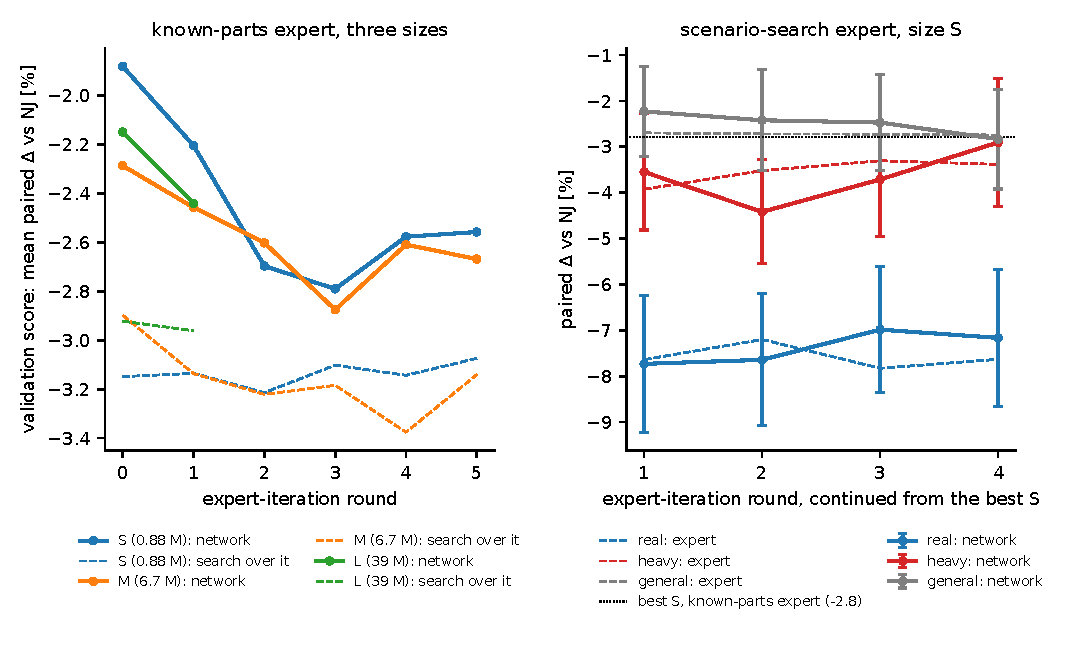
\includegraphics[width=\linewidth]{figures/training.pdf}
\caption{Left: validation score (mean paired $\Delta$ vs \nj\ over the three groups) per
expert-iteration round for the three sizes with the known-parts expert (solid: network
alone; dashed: the search over it). Right: the S network continued with the scenario
search as expert, per group (network alone with 95\,\% CIs; dashed: its expert); the dotted
line is the best S score with the known-parts expert.}
\label{fig:training}
\end{figure}

\subsection{The scenario search improves on the known-parts expert}\label{sec:sf}
Continuing the best S network with the scenario search as expert (Table~\ref{tab:sfruns},
Figure~\ref{fig:training} right) moved the score from $-2.79$ to $-4.50$\,\% after one
iteration and $-4.83$\,\% after two: $-7.6$\,\% on the reference cell, $-4.4$\,\% on the
heavy variant and $-2.4$\,\% on the general cells, at the same 4~ms per decision. From the
second iteration the network alone is at or above the search over itself on the reference
and heavy cells ($-7.6$ against $-7.2$, $-4.4$ against $-3.5$): the search is noisy (eight
sampled futures) and the network learns its average. Two further continuations changed the
training set rather than the method: the design mode with its corrected tokens and the
three observation levels (score $-3.98$\,\% in the design mode, where the \nj\ baseline
already pre-positions), and bursty arrivals with slow heads in the mix (score $-3.82$\,\%
over four groups). No difference between the last network and the previous one was detected head to
head ($+0.47\pm0.69$, $-0.36\pm0.83$, $+0.20\pm0.48$ and $+0.09\pm0.36$\,\% on the four
groups): extending the training to the declared scope produced no detectable improvement,
and the owner froze that network (iteration~1) for the confirmatory run.

\begin{table}[t]
\centering\small
\caption{Expert iteration with the scenario search, size S: per iteration, the network
alone on the validation groups (paired $\Delta$ vs \nj\ [\%, 95\,\% CI]), its score and
its expert's score. Bold iterations were accepted. The first run validates in the basic
mode; the two continuations in the design mode (where \nj\ also pre-positions), with the
fourth group added in the last. Legacy tie-break.}
\label{tab:sfruns}
\resizebox{\linewidth}{!}{% generated by experiments/paper1_figures.py
\begin{tabular}{@{}llcccccc@{}}
\toprule
run & it. & net real & net heavy & net general & net real/bursts & score & teacher score \\
\midrule
\multicolumn{8}{@{}l}{\texttt{rl2\_gen\_s\_sf}: sampled-future teacher, from \texttt{rl2\_gen\_s\_big}; `none'} \\
 & \textbf{1} & $-7.73 \pm 1.49$ & $-3.55 \pm 1.26$ & $-2.23 \pm 0.98$ & --- & -4.50 & -4.75 \\
 & \textbf{2} & $-7.64 \pm 1.44$ & $-4.42 \pm 1.13$ & $-2.42 \pm 1.10$ & --- & -4.83 & -4.48 \\
 & 3 & $-6.99 \pm 1.38$ & $-3.71 \pm 1.25$ & $-2.47 \pm 1.05$ & --- & -4.39 & -4.62 \\
 & 4 & $-7.16 \pm 1.48$ & $-2.91 \pm 1.40$ & $-2.83 \pm 1.09$ & --- & -4.30 & -4.59 \\
\multicolumn{8}{@{}l}{\texttt{rl2\_gen\_s\_d}: + design mode, corrected tokens, observation levels; from \texttt{s\_sf}} \\
 & \textbf{1} & $-6.40 \pm 1.50$ & $-2.04 \pm 1.28$ & $-3.08 \pm 1.08$ & --- & -3.84 & -4.15 \\
 & \textbf{2} & $-6.61 \pm 1.40$ & $-2.45 \pm 1.20$ & $-2.88 \pm 1.07$ & --- & -3.98 & -4.35 \\
 & 3 & $-6.67 \pm 1.36$ & $-2.40 \pm 1.32$ & $-2.87 \pm 1.06$ & --- & -3.98 & -4.00 \\
 & 4 & $-6.37 \pm 1.43$ & $-2.45 \pm 1.32$ & $-2.82 \pm 1.05$ & --- & -3.88 & -4.20 \\
\multicolumn{8}{@{}l}{\texttt{rl2\_gen\_s\_b}: + bursts and slow heads in the mix; from \texttt{s\_d}} \\
 & \textbf{1} & $-6.19 \pm 1.48$ & $-2.86 \pm 1.09$ & $-2.73 \pm 1.05$ & $-3.51 \pm 1.00$ & -3.82 & -4.09 \\
 & 2 & $-6.20 \pm 1.36$ & $-2.60 \pm 1.23$ & $-2.73 \pm 1.06$ & $-3.66 \pm 0.99$ & -3.80 & -3.98 \\
 & 3 & $-6.48 \pm 1.45$ & $-2.25 \pm 1.06$ & $-2.72 \pm 1.08$ & $-3.74 \pm 0.92$ & -3.80 & -3.99 \\
\bottomrule
\end{tabular}
}
\end{table}

\subsection{A burst-aware expert does not help}\label{sec:futures}
A network trained on bursty cells had not scored better than its expert, whose futures
are Poisson, so the natural next lever was an expert that samples the cell's on/off arrival model
(statistical knowledge of the process, started in its stationary state, not an
observation of the source's current state). Table~\ref{tab:futures} tests it on the
frozen network, the same realizations and the same budget. On Poisson cells the two
experts coincide by construction; on the bursty cell the burst-aware expert is half a
point \emph{worse} ($+0.52\pm0.49$\,\% paired against the Poisson one), and with strong
bursts no difference between the two was detected (intervals of $\pm0.4$--$0.6$\,\%). The stationary start adds to
every future the uncertainty of whether the source is emitting now, which eight futures
do not average out; the smoother Poisson future ranks the candidates with less noise. With
strong bursts the cell alternates between an idle head and a saturated burst, no expert
beats the network, and the known-parts order is close to what can be achieved without
seeing the hidden queue. The Poisson expert stays the expert of record.

\begin{table}[t]
\centering\small
\caption{Expert futures: the frozen network alone, and the scenario search over it with
Poisson futures and with the cell's on/off arrival model, on the validation groups
(design mode, 50 realizations per group, 100 general) and on two cells with strong
bursts (on 20\,\% of the time in 40~s periods). Paired $\Delta$ vs \nj\ [\%, 95\,\% CI]. Legacy tie-break.}
\label{tab:futures}
\resizebox{\linewidth}{!}{% generated by experiments/paper1_figures.py
\begin{tabular}{@{}lcccccc@{}}
\toprule
policy & real & heavy & general & real, bursts (0.3 / 20 s) & heavy, strong bursts (0.2 / 40 s) & real, strong bursts \\
\midrule
network alone & $-6.19 \pm 1.48$ & $-2.86 \pm 1.09$ & $-2.73 \pm 1.05$ & $-3.51 \pm 1.00$ & $-1.06 \pm 0.61$ & $-1.85 \pm 0.75$ \\
teacher, Poisson futures & $-6.44 \pm 1.30$ & $-2.35 \pm 1.46$ & $-3.51 \pm 1.27$ & $-4.07 \pm 0.96$ & $-1.13 \pm 0.58$ & $-1.60 \pm 0.71$ \\
teacher, cell futures & $-6.44 \pm 1.30$ & $-2.35 \pm 1.46$ & $-3.51 \pm 1.27$ & $-3.60 \pm 0.89$ & $-1.27 \pm 0.61$ & $-1.56 \pm 0.69$ \\
\bottomrule
\end{tabular}
}
\end{table}

\subsection{Learning from the reward: the earlier agents and the PPO baseline}\label{sec:rlhistory}
Before the representation of Section~\ref{M-sec:policy}, the project trained agents on 87
hand-made features with three slots per belt and an action restricted to the head of a
conveyor: behaviour cloning of the known-parts rollout, DAgger, and PPO fine-tuning with
action masks. On 30 development realizations of the reference cell in the basic mode the
cloned agent gave $-1.4$\,\% against \nj\ (not significant) and the PPO-tuned one
$+1.9$\,\%, worse than the rule; at the heavy load $-1.8$ and $-1.0$\,\%; longer PPO
training always made the cloned policy worse. Those results explain why the project
changed representation, action space and training scheme, but they do not answer the
question that matters now, since both the features and the actions differed.

\subsection{PPO baseline on the present representation}\label{sec:ppo}
\paragraph{Question and protocol.}
What does learning from the scenario search add over learning directly from the reward,
with the same tokens, the same action mask (non-candidates excluded, single-candidate
decisions taken without the network), the same event-driven simulator, the same network
(size S, 0.88~M parameters) and the same cell distribution as the policy of
Section~\ref{M-sec:policy}? A policy-gradient baseline \cite{Schulman2017} answers it in
two variants, both under a protocol fixed and committed before the runs and not changed
afterwards (the project's methods documentation records it, together with a smoke test
run before freezing): \textbf{V1}, PPO \emph{from scratch}; \textbf{V2}, PPO as a
\emph{fine-tuning of the learned policy}, initialized from the frozen network and its
value scale. Reward per decision equal to minus the increase of the penalized objective
between decisions, $\gamma=1$ (finite drained episodes), GAE with $\lambda=0.95$,
clipping 0.2, four epochs per update, minibatches of 256 decisions, entropy coefficient
0.01, value coefficient 0.5, AdamW at $3\cdot10^{-4}$; one update per batch of 1\,000
episodes; V1 with a budget of 40\,000 training episodes per run, comparable to the
36\,000 acting episodes of the expert-iteration chain that produced the frozen network,
and V2 with 12\,000; three training seeds per variant (200\,000+, disjoint from the
expert-iteration seeds); checkpoints every 4\,000 episodes scored greedily on the
validation groups with the scoring of expert iteration, the best kept; evaluation paired
on the same development realizations against \nj\ and against the frozen network, per
seed and as the mean over seeds, with 95\,\% intervals; and the training cost of both
schemes. The reserved realizations are not used: the checkpoints are selected and compared on
the same development validation realizations as the expert-iteration chain, so this
section is development evidence, like the rest of Section~\ref{M-sec:dev}; the
comparisons that used reserved realizations are those of Section~\ref{M-sec:confirm}. The
improvement is decided by the evaluation performance and the training cost; a larger
approximate KL per update means that the policy changed more during training, nothing
else.

\paragraph{V1: PPO from scratch.}
Table~\ref{tab:ppo_v1} and Figure~\ref{fig:ppo} (left). No run reaches \nj\ within the
budget: the selected checkpoints score $+3.62$, $+4.49$ and $+7.88$\,\% above the rule
(mean over seeds $+5.33$\,\%), where the frozen network scores $-3.82$\,\% on the same
realizations; against the frozen network they are $+7.89$ to $+12.31$\,\% worse (mean
$+9.66$\,\%) and lose on every group with every seed (at most 12 wins of 100 on the
general cells, at most 6 of 50 elsewhere). The reference cell at the nominal load is the
one group where no difference between PPO and the rule was detected ($-0.09$ to $+1.32$\,\%, intervals containing 0);
the heavy load is the hardest ($+9.1$ to $+19.6$\,\%). Two of the three runs select
their last checkpoint and are still improving at 40\,000 episodes, by about 0.5--1
point per 4\,000 episodes; the training signal is healthy to the end (entropy from
1.8 to 0.8--1.0 nats, approximate KL per update 0.003--0.016, clipped fraction
2--15\,\%, the mean sampled training cost falling from 83--92 to 49--52~s per part). The
curves do not say what a larger budget would have given; the defensible result is what
each method reached with the budget used. One seed
behaves differently: its greedy score is best at 16\,000 episodes and worsens afterwards
while its sampled training cost keeps falling. Scoring its checkpoints with both
decodings, a post hoc diagnosis, shows why: the sampled policy, the one PPO optimizes, improves from $+47.9$ to
$+26.4$\,\% above \nj\ between 16\,000 and 40\,000 episodes while its greedy mode goes
from $+7.9$ to $+11.6$\,\%; the policies are still far from deterministic at the end of
the budget, their sampled score is 15--40 points worse than their greedy score (the
frozen network's two decodings are one point apart, $-2.80$ against $-3.82$\,\%), and
greedy decoding is the favourable one for PPO, so the comparison above holds under
either decoding.

\begin{table}[t]
\centering
\caption{V1, PPO from scratch: paired evaluation of the selected checkpoints on the
validation groups (design mode, 50 realizations per group, 100 general cells; greedy
decoding). Paired $\Delta$ vs \nj\ and vs the frozen expert-iteration network [\%, 95\,\% CI,
wins out of $n$]; score = mean of the four groups. The frozen network's row reproduces
Table~\ref{tab:sfruns}.}
\label{tab:ppo_v1}
\resizebox{\linewidth}{!}{% generated by experiments/paper1_figures.py
\begin{tabular}{@{}llccccc@{}}
\toprule
policy & best checkpoint & real & heavy & general & real/bursts & score \\
\midrule
\multicolumn{7}{@{}l}{\emph{vs \nj}} \\
\texttt{rl2\_gen\_s\_b} (expert iteration, frozen) & --- & $-6.19 \pm 1.48$ (46/50) & $-2.86 \pm 1.09$ (38/50) & $-2.73 \pm 1.05$ (49/100) & $-3.51 \pm 1.00$ (42/50) & -3.82 \\
\texttt{rl2\_ppo\_s0} & update 40 (40,000 ep.) & $+0.71 \pm 1.74$ (22/50) & $+10.49 \pm 2.24$ (4/50) & $+3.64 \pm 1.99$ (21/100) & $+3.11 \pm 1.46$ (14/50) & +4.49 \\
\texttt{rl2\_ppo\_s1} & update 16 (16,000 ep.) & $+1.32 \pm 1.99$ (21/50) & $+19.59 \pm 2.70$ (1/50) & $+7.19 \pm 2.32$ (11/100) & $+3.44 \pm 1.39$ (12/50) & +7.88 \\
\texttt{rl2\_ppo\_s2} & update 40 (40,000 ep.) & $-0.09 \pm 1.42$ (27/50) & $+9.09 \pm 1.59$ (3/50) & $+3.13 \pm 1.72$ (22/100) & $+2.32 \pm 1.38$ (18/50) & +3.62 \\
mean over seeds & & $+0.65 \pm 1.47$ (21/50) & $+13.06 \pm 1.67$ (0/50) & $+4.65 \pm 1.82$ (16/100) & $+2.96 \pm 1.31$ (13/50) & +5.33 \\
\midrule
\multicolumn{7}{@{}l}{\emph{vs \texttt{rl2\_gen\_s\_b} (negative = PPO better)}} \\
\texttt{rl2\_ppo\_s0} & & $+7.53 \pm 1.94$ (4/50) & $+13.88 \pm 2.50$ (3/50) & $+6.77 \pm 2.17$ (9/100) & $+6.96 \pm 1.64$ (3/50) & +8.78 \\
\texttt{rl2\_ppo\_s1} & & $+8.16 \pm 2.09$ (3/50) & $+23.17 \pm 2.65$ (0/50) & $+10.61 \pm 2.81$ (6/100) & $+7.30 \pm 1.64$ (3/50) & +12.31 \\
\texttt{rl2\_ppo\_s2} & & $+6.68 \pm 1.61$ (4/50) & $+12.41 \pm 1.69$ (1/50) & $+6.33 \pm 2.09$ (12/100) & $+6.14 \pm 1.60$ (6/50) & +7.89 \\
mean over seeds & & $+7.46 \pm 1.61$ (3/50) & $+16.48 \pm 1.76$ (0/50) & $+7.90 \pm 2.19$ (8/100) & $+6.80 \pm 1.53$ (3/50) & +9.66 \\
\bottomrule
\end{tabular}
}
\end{table}

\paragraph{V2: PPO as a fine-tuning of the learned policy.}
Table~\ref{tab:ppo_v2} and Figure~\ref{fig:ppo} (right). Initialized from the frozen
network (its initial validation reproduces the $-3.82$\,\% exactly), fine-tuning with
the reward makes the policy worse on all three seeds: the best checkpoint is the first
one (4\,000 episodes) on every seed, at $-2.26$, $-3.22$ and $-2.73$\,\% against \nj,
and the later checkpoints are worse or equal ($-1.17$, $-1.69$ and $-2.47$\,\% at
12\,000). Against the frozen network the selected checkpoints are $+0.67$ to
$+1.72$\,\% worse (mean $+1.20$\,\%, 12--21 wins of 50 and 20 of 100 on the general
cells), on every group. The first update already moves the policy far from the
initialization: approximate KL 0.06--0.07 at the first update and 0.08--0.15 at the
second, clipped fraction 21--25\,\%, against 0.003 and 2\,\% at the first update from
scratch; the entropy rises from 0.43--0.48 to 0.5--0.65 nats and the sampled training
cost rises over the run. The cost-to-go of PPO's first batches matches the loaded value
scale of the frozen network, so the degradation is not a mismatch of the value target.
Within the frozen protocol (the same step size as V1, no penalty towards the
initialization), the reward signal does not improve the amortized policy of the search;
the answer to the fine-tuning question is no at this step size.

\begin{table}[t]
\centering
\caption{V2, PPO fine-tuning of the learned policy (initialized from the frozen network,
12\,000 episodes, three seeds): paired evaluation of the selected checkpoints, as
Table~\ref{tab:ppo_v1}.}
\label{tab:ppo_v2}
\resizebox{\linewidth}{!}{% generated by experiments/paper1_figures.py
\begin{tabular}{@{}llccccc@{}}
\toprule
policy & best checkpoint & real & heavy & general & real/bursts & score \\
\midrule
\multicolumn{7}{@{}l}{\emph{vs \nj}} \\
\texttt{rl2\_gen\_s\_b} (expert iteration, frozen) & --- & $-6.19 \pm 1.48$ (46/50) & $-2.86 \pm 1.09$ (38/50) & $-2.73 \pm 1.05$ (49/100) & $-3.51 \pm 1.00$ (42/50) & -3.82 \\
\texttt{rl2\_ppo\_ft\_s3} & update 4 (4,000 ep.) & $-3.77 \pm 1.46$ (39/50) & $-1.30 \pm 1.15$ (32/50) & $-1.73 \pm 0.97$ (44/100) & $-2.25 \pm 0.95$ (37/50) & -2.26 \\
\texttt{rl2\_ppo\_ft\_s4} & update 4 (4,000 ep.) & $-5.59 \pm 1.64$ (43/50) & $-2.03 \pm 1.15$ (34/50) & $-2.44 \pm 1.08$ (50/100) & $-2.81 \pm 0.94$ (40/50) & -3.22 \\
\texttt{rl2\_ppo\_ft\_s5} & update 4 (4,000 ep.) & $-4.67 \pm 1.56$ (40/50) & $-2.22 \pm 1.23$ (36/50) & $-1.45 \pm 0.90$ (40/100) & $-2.59 \pm 0.90$ (39/50) & -2.73 \\
mean over seeds & & $-4.68 \pm 1.40$ (43/50) & $-1.85 \pm 0.96$ (38/50) & $-1.87 \pm 0.91$ (48/100) & $-2.55 \pm 0.86$ (39/50) & -2.74 \\
\midrule
\multicolumn{7}{@{}l}{\emph{vs \texttt{rl2\_gen\_s\_b} (negative = PPO better)}} \\
\texttt{rl2\_ppo\_ft\_s3} & & $+2.68 \pm 1.23$ (11/50) & $+1.71 \pm 1.32$ (18/50) & $+1.12 \pm 0.71$ (19/100) & $+1.35 \pm 0.81$ (11/50) & +1.72 \\
\texttt{rl2\_ppo\_ft\_s4} & & $+0.67 \pm 1.05$ (21/50) & $+0.94 \pm 1.18$ (24/50) & $+0.33 \pm 0.60$ (26/100) & $+0.76 \pm 0.64$ (14/50) & +0.67 \\
\texttt{rl2\_ppo\_ft\_s5} & & $+1.73 \pm 1.42$ (19/50) & $+0.70 \pm 1.02$ (21/50) & $+1.43 \pm 0.74$ (14/100) & $+1.00 \pm 0.72$ (14/50) & +1.22 \\
mean over seeds & & $+1.69 \pm 1.02$ (14/50) & $+1.12 \pm 0.95$ (21/50) & $+0.96 \pm 0.55$ (20/100) & $+1.04 \pm 0.62$ (12/50) & +1.20 \\
\bottomrule
\end{tabular}
}
\end{table}

\begin{figure}[t]
\centering
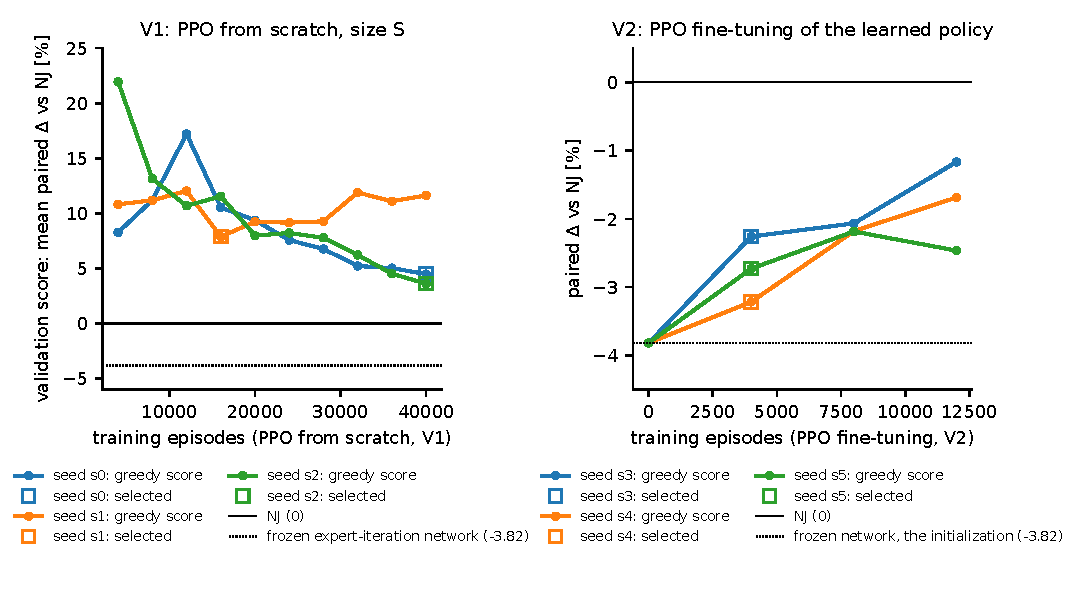
\includegraphics[width=\linewidth]{figures/ppo.pdf}
\caption{Validation score (mean paired $\Delta$ vs \nj\ over the four groups, greedy
decoding) against training episodes. Left: V1, PPO from scratch, three seeds; the
random initialization (update 0, $+37$ to $+78$\,\%) is above the axis. Right: V2, PPO
fine-tuning of the learned policy, three seeds, starting at the frozen network's
$-3.82$\,\%. Hollow squares: the selected checkpoints.}
\label{fig:ppo}
\end{figure}

\paragraph{Training cost and latency.}
Table~\ref{tab:ppo_cost}. One V1 run takes 22~minutes of wall-clock on 40 workers (6
in generation, 15 in the GPU updates), an upper bound of 14.5 CPU-hours; the
expert-iteration chain that produced the frozen network took 12.7~hours on 47 workers,
an upper bound of 596 CPU-hours, 90\,\% of it in generation, where the expert's
look-ahead runs about 39~million partial-episode clones (known-parts expert, 4.1 clone
runs per labelled decision; scenario-search expert, 32.8, measured on a sample of 40
episodes per setting and scaled by the logged labelled decisions). The clearest
comparison is the wall-clock on the same workstation: 22~minutes for one PPO run against
12.7~hours for the whole chain, at a comparable number of acting episodes, with the
chain's extra time in the expert's look-ahead; the CPU-hour figures are upper bounds
computed as wall-clock times workers, not measured consumption, and are given to state
the scope of the comparison, not as a ratio. The V2 runs take 6~minutes each. The PPO checkpoint has the latency of the network it is (same
architecture, 884\,994 parameters): 1.06~ms per decision for a single state on one
thread, against 1.06~ms for an untrained network of the same size on the same machine,
so the comparison with expert iteration is at equal inference cost. The 4.1~ms median of Section~\ref{M-sec:policy} was measured on a different machine.

\begin{table}[t]
\centering
\caption{Training cost of the PPO baseline and of the expert-iteration chain
(\texttt{rl2\_gen\_s\_big} to \texttt{rl2\_gen\_s\_b}) on the same workstation. CPU-h is the
upper bound wall-clock $\times$ workers; the GPU column is the time in the policy
updates; the look-ahead clone runs of the chain are estimated from the logged labelled
decisions and a measured sample (partial episodes, not full ones). Best score = greedy
validation score vs \nj\ [\%].}
\label{tab:ppo_cost}
\resizebox{\linewidth}{!}{% generated by experiments/paper1_figures.py
\begin{tabular}{@{}lrrrrrrr@{}}
\toprule
run & wall-clock & workers & CPU-h (wall $\times$ workers) & GPU updates & acting episodes & look-ahead clone runs & best score \\
\midrule
\texttt{rl2\_ppo\_s0} (PPO from scratch) & 22 min & 40 & 14.5 & 15 min & 40,000 & 0 & +4.49 \\
\texttt{rl2\_ppo\_s1} (PPO from scratch) & 22 min & 40 & 14.7 & 16 min & 40,000 & 0 & +7.88 \\
\texttt{rl2\_ppo\_s2} (PPO from scratch) & 22 min & 40 & 14.4 & 15 min & 40,000 & 0 & +3.62 \\
\midrule
\texttt{rl2\_gen\_s\_big} (known-parts expert, 6 it.) & 0.40 h & 47 & 19 & 7 min & 14,000 & 2.8 M & -2.79 \\
\texttt{rl2\_gen\_s\_sf} (sampled-future expert, 4 it.) & 3.87 h & 47 & 182 & 3 min & 8,000 & 12.8 M & -4.83 \\
\texttt{rl2\_gen\_s\_d} (sampled-future expert, 4 it.) & 4.34 h & 47 & 204 & 4 min & 8,000 & 13.0 M & -3.98 \\
\texttt{rl2\_gen\_s\_b} (sampled-future expert, 3 it.) & 4.08 h & 47 & 192 & 3 min & 6,000 & 10.3 M & -3.82 \\
expert-iteration chain, total & 12.7 h & & 596 & 17 min & 36,000 & 38.9 M & \\
\bottomrule
\end{tabular}
}
\end{table}

\paragraph{Reading.}
Under the protocols tried, the chain trained with the search performed better: with the
same architecture and a comparable number of acting episodes, learning from the reward
alone gave a policy 8--12\,\% worse than the one learned from the search and 4--8\,\%
worse than the dispatching rule that the search-trained policy beats by 3.8\,\%, in
22~minutes per run against 12.7~hours for the chain. The two methods share the
architecture, the mask, the simulator and the evaluation groups and differ in three
things the experiment does not separate: the learning signal (labels of a search
against the reward), the compute spent (the chain's look-ahead), and the curriculum
(the chain's stages change the training mix, the design mode and corrected inputs at
one stage and bursty arrivals and slow heads at the next, while PPO trains on the
final mix from the first episode).
Fine-tuning the search-trained policy with the reward did not improve it. The PPO
checkpoints were selected and compared on the same validation realizations, so this is
development evidence; the confirmatory comparisons are those of Section~\ref{M-sec:confirm}.
Not done, and listed as the limits of this baseline: a hyperparameter search, reward
shaping, a penalty towards the initialization in V2, and longer budgets.

%====================================================================
\section{Confirmatory evaluation: complements}\label{sec:confirmfull}
%====================================================================
\subsection{Protocol (full text)}
The frozen network, the known-parts search over \nj, the scenario search over the
frozen network (``its expert'' below: the search built on the final network, not the
searches over earlier networks that labelled its training data), \nj\ and \nh\ were run on 30 realizations reserved for this
evaluation (seeds 7000--7029; the companion paper analyzes the same phase-4 realizations
for different research questions), never seen by any design decision and used once, on eight
regimes: the reference cell and its heavy variant, Poisson and bursty arrivals, nominal
head and a head twice as slow (Table~\ref{tab:regimes}), in the basic mode (B) and in the
design mode (C). Every policy runs on the same realizations (common random numbers), so
every contrast is a paired difference; we report $\Delta=100\,(\frac{1}{30}\sum_\omega
J_X(\omega)/J_Y(\omega)-1)$ for ``X vs Y'', negative favouring $X$, with a normal 95\,\%
interval and, for the contrasts between policies, the number of realizations in which $X$
is cheaper. Latencies are measured on the decisions of the network's episodes: at every
decision with at least two candidates, every policy is timed on the same state (one
thread, the machine fully loaded by the other workers), 16\,215 decisions in B and
17\,147 in C. The protocol, the regimes and the contrasts were fixed before the run; the
per-episode results and the per-decision latencies are distributed with the source.
The run used the legacy arrival-time tie-break for \nj, \nh\ and the known-parts search
(Section~\ref{M-sec:online}): their numbers below are those of comparators run under
that key, whose effect on development realizations was at most $\pm1.5$\,\% per
regime and of either sign. After the run, as a retrospective sensitivity analysis and
not as a new confirmation, \nj, \nh\ and the known-parts search (with the key applied
both to the candidate ranking and inside every look-ahead continuation) were rerun on the
same reserved realizations with both keys (every legacy rerun reproduces the archived
cost, the largest difference being $1.4\cdot10^{-13}$~s per part) and paired with the
archived costs of the network (results below). These reruns reuse the reserved
realizations; a confirmation of the margins under the observable key would need fresh
ones.

\begin{table}[t]
\centering\small
\caption{Regimes of the confirmatory evaluation and their physical scales ($\tcross$ is
the head's travel time across the conveyors); parts, penalized flow time, flow time,
blocking events and blocked conveyor-seconds are means per episode for \nj\ in B over the
30 realizations (seeds 7000--7029, the phase-4 realizations that the companion paper also
analyzes).}
\label{tab:regimes}
\resizebox{\linewidth}{!}{% generated by experiments/paper1_figures.py
\begin{tabular}{@{}lcccccccc@{}}
\toprule
regime & belt [cm/s] & head [cm/s] & $\tau_{\mathrm{cross}}$ [s] & parts & $J$ (\textsc{nj}, B) [s/part] & flow [s] & blocking events & blocked [belt-s] \\
\midrule
real / Poisson / nominal head & 3 & 10 & 2.4 & 78 & 21.8 & 19.3 & 7.8 & 122 \\
real / Poisson / slow head & 3 & 5 & 4.8 & 78 & 42.1 & 36.1 & 14.8 & 322 \\
real / bursts / nominal head & 3 & 10 & 2.4 & 73 & 27.6 & 25.8 & 5.1 & 93 \\
real / bursts / slow head & 3 & 5 & 4.8 & 73 & 41.3 & 37.8 & 8.2 & 184 \\
heavy / Poisson / nominal head & 5 & 5 & 4.8 & 94 & 73.5 & 65.2 & 18.2 & 601 \\
heavy / Poisson / slow head & 5 & 2.5 & 9.6 & 94 & 104.0 & 94.7 & 14.2 & 720 \\
heavy / bursts / nominal head & 5 & 5 & 4.8 & 89 & 72.0 & 66.4 & 11.1 & 399 \\
heavy / bursts / slow head & 5 & 2.5 & 9.6 & 89 & 93.6 & 87.0 & 9.1 & 508 \\
\bottomrule
\end{tabular}
}
\end{table}

\subsection{Results (full text)}
Figure~\ref{fig:confirm} shows the contrasts of Tables~\ref{M-tab:confirmB} and \ref{M-tab:confirmC} graphically.

\begin{figure}[t]
\centering
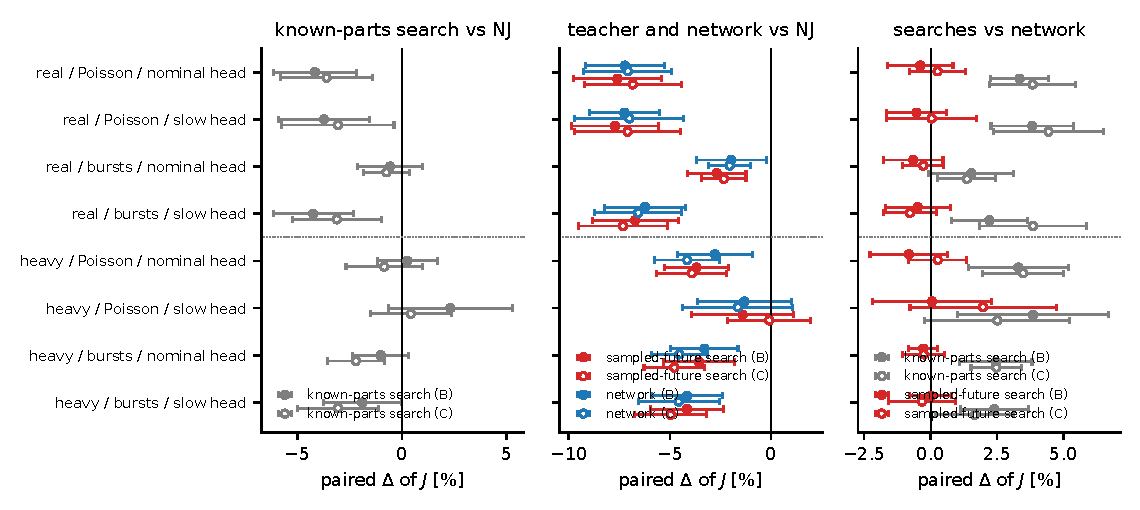
\includegraphics[width=\linewidth]{figures/confirm.pdf}
\caption{Confirmatory evaluation on the eight regimes (paired $\Delta$ of the penalized
flow time, 95\,\% CI; filled markers: basic mode B, hollow: design mode C). Left: the
known-parts search against \nj. Middle: the scenario search (expert) and the network
against \nj. Right: the two searches against the network (positive = the network is
better). Rules and known-parts search with the legacy tie-break; seeds 7000--7029, shared
with the companion paper.}
\label{fig:confirm}
\end{figure}
\textbf{The network alone beats \nj\ in seven of the eight regimes} (legacy key; in all
eight under the observable key, below), by 2.0--7.3\,\% in B
($-7.2$ and $-7.3$\,\% on the reference cell with Poisson arrivals, $-2.0$ and $-6.2$ with
bursts, $-2.8$ to $-4.2$ at the heavy load) and by 2.0--7.1\,\% in C; the exception is the
heavy load with Poisson arrivals and a slow head ($-1.3\pm2.3$ and $-1.6\pm2.7$), where
with every belt queueing and a head at 2.5~cm/s no tested policy improved on the
nearest-part rule by a detectable amount; how far all of them are from the optimum is
not measured. The intervals are individual: Holm's adjustment over the eight regimes of
each mode leaves six detections in B and seven in C. With \nj\ rerun under the observable
tie-break (retrospective, same realizations, network costs unchanged), the network is
cheaper with an individual interval excluding zero in all eight regimes in both modes
(2.0--7.6\,\% in B and 2.1--7.6\,\% in C); in the exception above the contrasts become
$-2.1\pm2.0$ and $-2.7\pm2.5$, so the margin there stays close to zero. Under the
observable key the known-parts search costs more than the network in all sixteen
regime--mode comparisons, 1.4--4.7\,\% in B and 1.5--5.2\,\% in C, with an individual
interval excluding zero in seven regimes in B and eight in C (the same counts after Holm);
pooled over the regimes it costs $2.95$\,\% more in B $[2.24,3.66]$ and $3.21$\,\% more in C
$[2.38,4.04]$. \nh\ under the observable key costs 1.4--8.2\,\% more than the network in B
and 1.5--6.7\,\% in C, with an individual interval excluding zero in six regimes in B and
seven in C (six and six after Holm). These two contrasts are
$100\,(J_{\mathrm{comparator}}/J_{\mathrm{network}}-1)$, positive favouring the network; the
paired costs are distributed with the source in \texttt{data/closure\_0\_7\_40} and the
scripts in \texttt{experiments/closure\_0\_7\_40}.

\textbf{It has a lower cost than the known-parts search in every regime} (legacy key; the
observable-key rerun is above): the search costs 1.5--3.9\,\% more than the policy in B and
1.4--4.4 in C, significantly in seven of eight in both modes, at 2--3 times the search's
latency. At the heavy load with Poisson arrivals in B the known-parts search shows no detected
improvement over \nj\ (point estimates $+0.3$ and $+2.3$\,\%, intervals containing zero):
the look-ahead over the parts in view, without the sampled future, is not better than
the rule when every belt is queueing, and whether it is worse is not resolved by these
intervals.

\textbf{No difference from its expert was detected} (no equivalence margin was set, so
this is not a test of equivalence). The paired contrast of the
scenario search over the network against the network alone includes zero in every
regime and mode, with point estimates within $\pm0.8$\,\% in B, and in C within $\pm0.8$\,\% except
the heavy load with Poisson arrivals and a slow head, where the point estimate favours
the network by $2.0\pm2.8$\,\%, an interval that admits a practically relevant difference (the intervals are wider than
the point estimates throughout); the search is cheaper in 12--18 of the 30
realizations, at 0.4--1.9~s per decision
(median by regime; 1.2~s pooled, 3.6~s at the 95th percentile, 12~s at most; 2\,600
look-aheads per episode on average). No difference between the amortized policy and
the search was detected, at about 1/100 of the search's latency, on reserved
realizations, which is what every development run had shown on the validation cells.

\textbf{Latency.} Pooled over the regimes, the network decides in 10.8~ms (median),
17.5~ms (95th percentile), 25.5~ms (99th) and 106~ms at most, on one thread with the
machine fully loaded by 47 other workers (Figure~\ref{fig:latency}); the 4~ms of
Section~\ref{M-sec:policy} is the same model on an unloaded machine. Against the design's
5~ms budget, on the loaded machine the network exceeded it in 98.07\,\% of the 16\,215
decisions of B and in 97.62\,\% of the 17\,147 of C, the known-parts search in 48.25 and
45.72\,\%, the scenario search in every decision, \nh\ in none, and \nj\ in one decision
of C (9.9~ms; 1 of 17\,147, 0.006\,\%) and none of B; on the unloaded
machine the only figure available is the 4.1~ms median, which does not establish a
per-decision guarantee. The physical slack of
the cell, the time until the next part reaches $b$, is seconds, three orders of magnitude
above either figure. The known-parts search decides in 4.8~ms (16~ms at the 95th
percentile) and the rules in under 0.2~ms.
\begin{figure}[t]
\centering
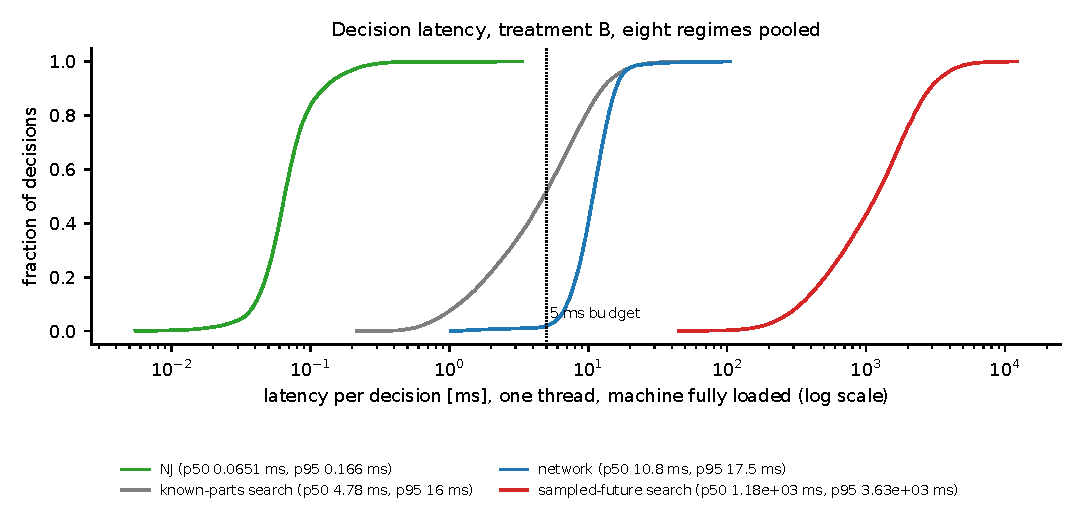
\includegraphics[width=\linewidth]{figures/latency.pdf}
\caption{Empirical distribution of the per-decision latency of the four policies on the
same decisions (basic mode, eight regimes pooled, seeds 7000--7029, shared with the
companion paper, one thread, machine fully loaded; log scale). The dotted line is the 5~ms budget of the design: on this loaded machine the
network exceeded it in 98.1\,\% of the decisions in B and 97.6\,\% in C (10.8~ms median);
on an unloaded machine the available figure is a median of 4.1~ms, not a per-decision
guarantee.}
\label{fig:latency}
\end{figure}

\textbf{Design mode.} With pre-positioning allowed to every policy, the picture is the
same; the network's margin over \nj\ is smaller at the reference load, because \nj\ itself
gains 7.4\,\% from pre-positioning there (Paper~2), and larger at the heavy load with
bursts. The network's level in the design mode against \nj\ in the basic mode, the
plan's original target, is $-14.1$\,\% on the reference cell with Poisson arrivals
(target: at least $-10$\,\%).

%====================================================================
\section{Extended discussion}\label{sec:discussionfull}
%====================================================================
\subsection{What the formulation buys}
The odometer formulation makes the endogenous part of the problem explicit and cheap: a
part is one number, the belt is one monotone function, and interception, stops and
blocking are all consequences of the start times. It is what the exact simulator
implements event by event, what the MILP of Section~\ref{app:milp} discretizes, and what
the lower bounds exploit (the belt has advanced at most $v_k$ times the running time).
Its properties set the terms of the online problem: its offline maximum-lateness and
total-completion-time variants are strongly NP-hard with the number of conveyors in the
input, so exactness is for small windows; belt order is natural but not dominant, so the policy must
be free to point at any part; and under the sufficient conditions of light traffic every
non-idling ready-only rule makes the same decisions and is within one interception time
of the offline optimum, so the value of
a better decision rule is concentrated in the contended regimes, which is where the
confirmatory evaluation measures it.

\subsection{What the training runs show}
Three facts of Section~\ref{M-sec:dev} point the same way. Networks of 0.88, 6.7 and 39
million parameters scored $-2.79$, $-2.88$ and $-2.44$\,\% with the same expert in one
run each (size, episodes and iterations confounded), no difference detected; for every network no difference from its expert's score is detected after one or two iterations and then trades one validation group against
another; and after the switch to the scenario-search expert, a continuation of the best S
network in which the expert and further iterations changed together, the score moved by
about two points, where changing the size moved it by none. In the runs made, no detectable difference separated the amortized
policy from the search that labels its data, and the search scored better in the tested variants that score
every part, average more futures and do not truncate; these are observations on one
chain, not matched ablations of each component. The learned value
head, which would make deeper or cheaper search possible, is the part that failed: its
error is set by the randomness of the future, which no decision changes, and that error
swamps the differences between candidates. A value that predicted the \emph{difference}
between candidates rather than the cost-to-go might do better; we did not try it.

\subsection{What the policy cannot do}
The confirmatory run shows two limits of the problem rather than of the method. At the
heavy load with Poisson arrivals and a slow head, no policy beat the nearest-part rule with
its legacy tie-break by more than the noise (with bursts the policy does, by $4.2\pm1.7$ and
$4.6\pm2.0$\,\%; against the rule with the observable tie-break, rerun afterwards, the
network's margin there is $-2.1\pm2.0$ and $-2.7\pm2.5$\,\%, just excluding zero):
with every belt queueing, the order in which the visible parts are served matters little
and the hidden queue, which none of the policies sees, is what would matter (Paper~2
measures it at 2.7--3.7\,\%). With bursts the gain of deciding better falls to 2\,\% on
the reference cell, and an expert that knows the burst model does not raise it: the
information that would help, whether the source is on now, is not in the state.

\subsection{Limits}\label{sec:limits}
The distance to the optimum is not measured. The MILP of Section~\ref{app:milp} is a
formulation; the project's CP-SAT model implements its grid version for the makespan, the
mean flow time and the mean waiting time, and the penalized objective with (M12) is
specified but neither implemented nor validated against the continuous model, and a hindsight reference on the realized
instances was deferred to a second confirmatory run on new reserved realizations; the
lower bounds of Section~\ref{M-sec:bounds} have been compared with offline solutions on
small instances only, where part of the gap is the anticipation the rules cannot do. The
known-parts look-ahead is a rollout with $K=6$, not an exact search with the bounds as
pruning; since the level it reached was found low before the exact version was built, that search
remains a verification tool for the known-parts sub-problem. The policy-gradient baseline
of Section~\ref{sec:ppo} is one protocol at one budget, without a hyperparameter
search; it bounds what the reward alone gave here, not what it could give. The confirmatory
regimes are eight variants of one 3-belt cell; the general cells with one to six
conveyors appear only in the validation of training, on development realizations.
Latencies are for one CPU thread of a loaded workstation and a 0.88~M-parameter model.
Parts are points with a minimum spacing, the head has no acceleration, processing times
are constant in the confirmatory regimes, and the penalty weights are placeholders. The
reserved realizations were used once for the prespecified evaluation and reused afterwards
only for the retrospective reruns of its comparators.

\subsection{Conclusions of the full draft}
For a shared head over parallel conveyors whose belts stop for the head, the schedule
determines the availability of every part, and the problem this creates is strongly
NP-hard (offline, maximum lateness and total completion time, with the number of conveyors
in the input), naturally but not dominantly ordered by belt, and indifferent to the ready-only
rule under the sufficient conditions of light traffic, where every such non-idling rule
coincides within one interception time of the offline optimum in makespan and mean flow
time. In the contended regimes of a real cell, the decision that
serves the parts in view best is not the best decision: a look-ahead that samples the
unknown arrivals and scores the realized cost of every part decides better than the
nearest-part rule by 3--8\,\% of the penalized flow time in the seven significant regimes
of the basic mode (1.4--7.7\,\% over the eight) and than a look-ahead over the
known parts by 2--4\,\% of the cost in that mode (comparators with the legacy tie-break;
the scenario search itself was not rerun with the observable key), and a permutation-equivariant pointer policy trained by expert
iteration with that search as expert, on randomized cells, shows no detected difference
from it at a hundredth of its latency, 10~ms per decision on a loaded machine (above
the design's 5~ms budget on that machine). With the
tested expert and training runs, the larger networks did not score detectably better than the
0.88~M one; continuing the S network with the scenario-search expert did move the score
(expert and further iterations changed together). On reserved
realizations of eight regimes the policy beats the rule with its legacy tie-break in seven
(in all eight against the rule with the observable tie-break, rerun afterwards), and no difference
from its expert was detected in any. What remains open is how far all of this is
from the optimum: measuring a penalized optimality gap requires a reference validated
for that objective, which Section~\ref{app:milp} does not yet provide, on the realized
instances and a new set of reserved realizations; what learning from the reward
alone gives on the same representation was measured under one protocol, on development
realizations: PPO from scratch stayed 8--12\,\% behind the chain trained with the search
at a comparable number of episodes, in 22 minutes per run against 12.7 hours for the
chain (Section~\ref{sec:ppo}).

\bibliographystyle{plain}
\bibliography{../../literature/references,extra}

\end{document}
